\documentclass[11pt,a4paper,oldfontcommands]{memoir}
\usepackage[utf8]{inputenc}
\usepackage[T1]{fontenc}
\usepackage{microtype}
\usepackage[dvips]{graphicx}
\usepackage{xcolor}
\usepackage{times}
\usepackage{float}
\usepackage[french]{babel}
\usepackage{listings}
\usepackage[normalem]{ulem}
\useunder{\uline}{\ul}{}

\usepackage[
breaklinks=true,colorlinks=true,
%linkcolor=blue,urlcolor=blue,citecolor=blue,% PDF VIEW
linkcolor=black,urlcolor=black,citecolor=black,% PRINT
bookmarks=true,bookmarksopenlevel=2]{hyperref}

\usepackage{geometry}
% PDF VIEW
% \geometry{total={210mm,297mm},
% left=25mm,right=25mm,%
% bindingoffset=0mm, top=25mm,bottom=25mm}
% PRINT
\geometry{total={210mm,297mm},
left=20mm,right=20mm,
bindingoffset=10mm, top=25mm,bottom=25mm}

% Hide appendix sections
\usepackage[toc,page]{appendix}
\usepackage{etoolbox}
\appto\appendix{\addtocontents{toc}{\protect\setcounter{tocdepth}{0}}}

\OnehalfSpacing
%\linespread{1.3}

%%% CHAPTER'S STYLE
\chapterstyle{bianchi}
%\chapterstyle{ger}
%\chapterstyle{madsen}
%\chapterstyle{ell}
%%% STYLE OF SECTIONS, SUBSECTIONS, AND SUBSUBSECTIONS
\setsecheadstyle{\Large\bfseries\sffamily\raggedright}
\setsubsecheadstyle{\large\bfseries\sffamily\raggedright}
\setsubsubsecheadstyle{\bfseries\sffamily\raggedright}
\setlength{\parskip}{1em}

%%% STYLE OF PAGES NUMBERING
\pagestyle{plain}
\makepagestyle{plain}
\makeevenfoot{plain}{\thepage}{}{}
\makeoddfoot{plain}{}{}{\thepage}
\makeevenhead{plain}{}{}{}
\makeoddhead{plain}{}{}{}
\maxsecnumdepth{subsubsection}
\maxtocdepth{subsection}

\begin{document}
\begin{titlepage}

\newcommand{\HRule}{\rule{\linewidth}{0.5mm}}

\center
 
%----------------------------------------------------------------------------------------
%	HEADING SECTIONS
%----------------------------------------------------------------------------------------

\textsc{\LARGE Haute École d'ingénierie et de gestion \\du canton de Vaud}\\[1.5cm]
\textsc{\Large Projet de groupe (PDG)}\\[0.5cm]
\textsc{\large Rapport de projet}\\[0.5cm]

%----------------------------------------------------------------------------------------
%	TITLE SECTION
%----------------------------------------------------------------------------------------

\HRule \\[0.8cm]
{ \huge \bfseries LibreDraw}\\[0.4cm]
\HRule \\[1.5cm]
 
%----------------------------------------------------------------------------------------
%	AUTHOR SECTION
%----------------------------------------------------------------------------------------

\begin{minipage}{0.4\textwidth}
\begin{flushleft} \large
\emph{Auteurs:}\\
Sacha \textsc{Bron}\\
Yassin \textsc{Kammoun}\\
Paul \textsc{Ntawuruhunga}\\
Marc \textsc{Pellet}\\
David \textsc{Villa}
\end{flushleft}
\end{minipage}
~
\begin{minipage}{0.4\textwidth}
\begin{flushright} \large
\emph{Superviseur:} \\
Dr. René \textsc{Rentsch} 
\break 
\break 
\break 
\break 
\end{flushright}
\end{minipage}\\[4cm]

%----------------------------------------------------------------------------------------
%	DATE SECTION
%----------------------------------------------------------------------------------------

{\large \today}\\[3cm]

%----------------------------------------------------------------------------------------
%	LOGO SECTION
%----------------------------------------------------------------------------------------


\includegraphics[scale=0.3]{images/heigvd.png}
\hfill

\includegraphics[scale=0.6]{images/hesso.png}

\vfill

\end{titlepage}

\cleardoublepage
\tableofcontents*
\cleardoublepage
\listoffigures*
\cleardoublepage
\listoftables*
\cleardoublepage

%----------------------------------------------------------------------------------------
%	INTRODUCTION
%----------------------------------------------------------------------------------------

\chapter{Introduction}

Ce chapitre est une introduction de ce rapport de travail. Il s'agit dans un premier temps de rappeler le sujet du projet par une description complète de celui-ci. Viennent ensuite l'énumération, le commentaire et l'explication des objectifs que cherche à atteindre ce projet. Les technologies utilisées pour la réalisation du système sont introduites par la suite. Les différents membres constituant l'équipe de projet sont présentés. Cette introduction décrit précisément les rôles de chacun des protagonistes. Finalement, un commentaire quant à la décision de choisir un tel sujet de projet est exposé. Cela consiste à partager les motivations et les raisons qui ont poussé le groupe à partir sur un tel projet.

\section{Description du projet}

Le projet consiste en un outil de dessin tout à fait standard. Celui-ci permet entre autres de dessiner sur un espace de travail. Pour ce faire, l'utilisateur dispose d'un éventail d'outils:

\begin{itemize}
\item[$\bullet$] Outils de dessin: les outils de dessin mettent à disposition un crayon et une gomme permettant de dessiner sans restriction n'importe quelle forme géométrique.
\item[$\bullet$] Outils de formes: les outils de formes mettent à disposition un ensemble de formes géométriques prédéfinies pouvant être dessinées au sein d'un dessin et redimensionnées à la guise de l'utilisateur.
\item[$\bullet$] Outils de couleurs: les outils de couleurs mettent à disposition une palette de couleurs laquelle permet de définir la couleur du trait aussi bien pour les outils de dessin que pour les outils de formes.
\item[$\bullet$] Outils d'épaisseur: les outils d'épaisseur permettent de définir selon une liste prédéfinie l'épaisseur du trait aussi bien pour les outils de dessin que pour les outils de formes.
\end{itemize}

Malgré ce côté simpliste du système, celui-ci se démarque des outils de dessin traditionnels par le fait que l'espace de travail du dessinateur est non pas l'écran de l'utilisateur mais un support physique tel un mur, un sol, une table ou n'importe quelle autre surface susceptible de jouer le rôle de support de dessin. L'idéal est bien évidemment une surface plane. Toutefois, le système n'est pas restreint par une telle propriété. Celle-ci pourrait tout aussi bien être théoriquement abrupte, instable et biscornue. L'utilisateur définit lui-même ce qu'il juge être un support de dessin propice pour travailler.

\newpage

Le fait de dessiner sur un support physique plutôt que virtuel nécessite une substitution de la souris de l'ordinateur à un outil plus adéquat pour dessiner. Ceci est rendu possible par la mise à disposition d'un stylet au dessinateur. Ce stylet est conçu sur mesure par l'équipe de projet pour les besoins du système. Il reste toutefois un outil expérimental avec une casquette de prototype. En effet, celui-ci n'a pour but que de valider la conception et l'implémentation du système. Il n'en demeure pas moins que ce stylet reste relativement complexe pour accomplir une telle tâche.

Le stylet se présente sous la forme d'un stylo tout à fait usuel. Toutefois, de par l'objectif de son utilisation, il est caractérisé par les composants suivants:

\begin{itemize}
\item[$\bullet$] Une LED rouge.
\item[$\bullet$] Une LED verte.
\item[$\bullet$] Un interrupteur.
\item[$\bullet$] Une résistance.
\item[$\bullet$] Une batterie.
\item[$\bullet$] Un boîtier.
\end{itemize}

Bien que l'action de dessiner soit réalisée sur un support physique, le dessin à proprement parlé n'est pas gravé sur ce support. Les faits et gestes du dessinateur avec le stylet sont capturés par une caméra. Un programme informatique reçoit en permanence en provenance de cette caméra des informations liées aux faits et gestes du stylet manipulé par le dessinateur. C'est là qu'intervient le mécanisme du tracking, c'est-à-dire la détection et le suivi du stylet. Toutes ces informations récupérées sont communiqués à un autre programme informatique. Ce dernier stocke, analyse, traite et reproduit ces mêmes faits et gestes de manière à reconstituer logiquement et graphiquement le dessin correspondant.

Afin que le dessinateur puisse disposer d'un retour instantané de son dessin, un projecteur projette la reproduction fidèle du dessin réalisée au sein du second programme informatique. Ainsi, le dessinateur a l'illusion de dessiner directement sur son support physique. Il dispose en plus de cela des fonctionnalités usuelles de sérialisation de dessin. Il peut en effet enregistrer son travail et le reprendre ultérieurement.

La figure suivante illustre un exemple d'environnement de dessin :

\begin{figure}[h]
\centering
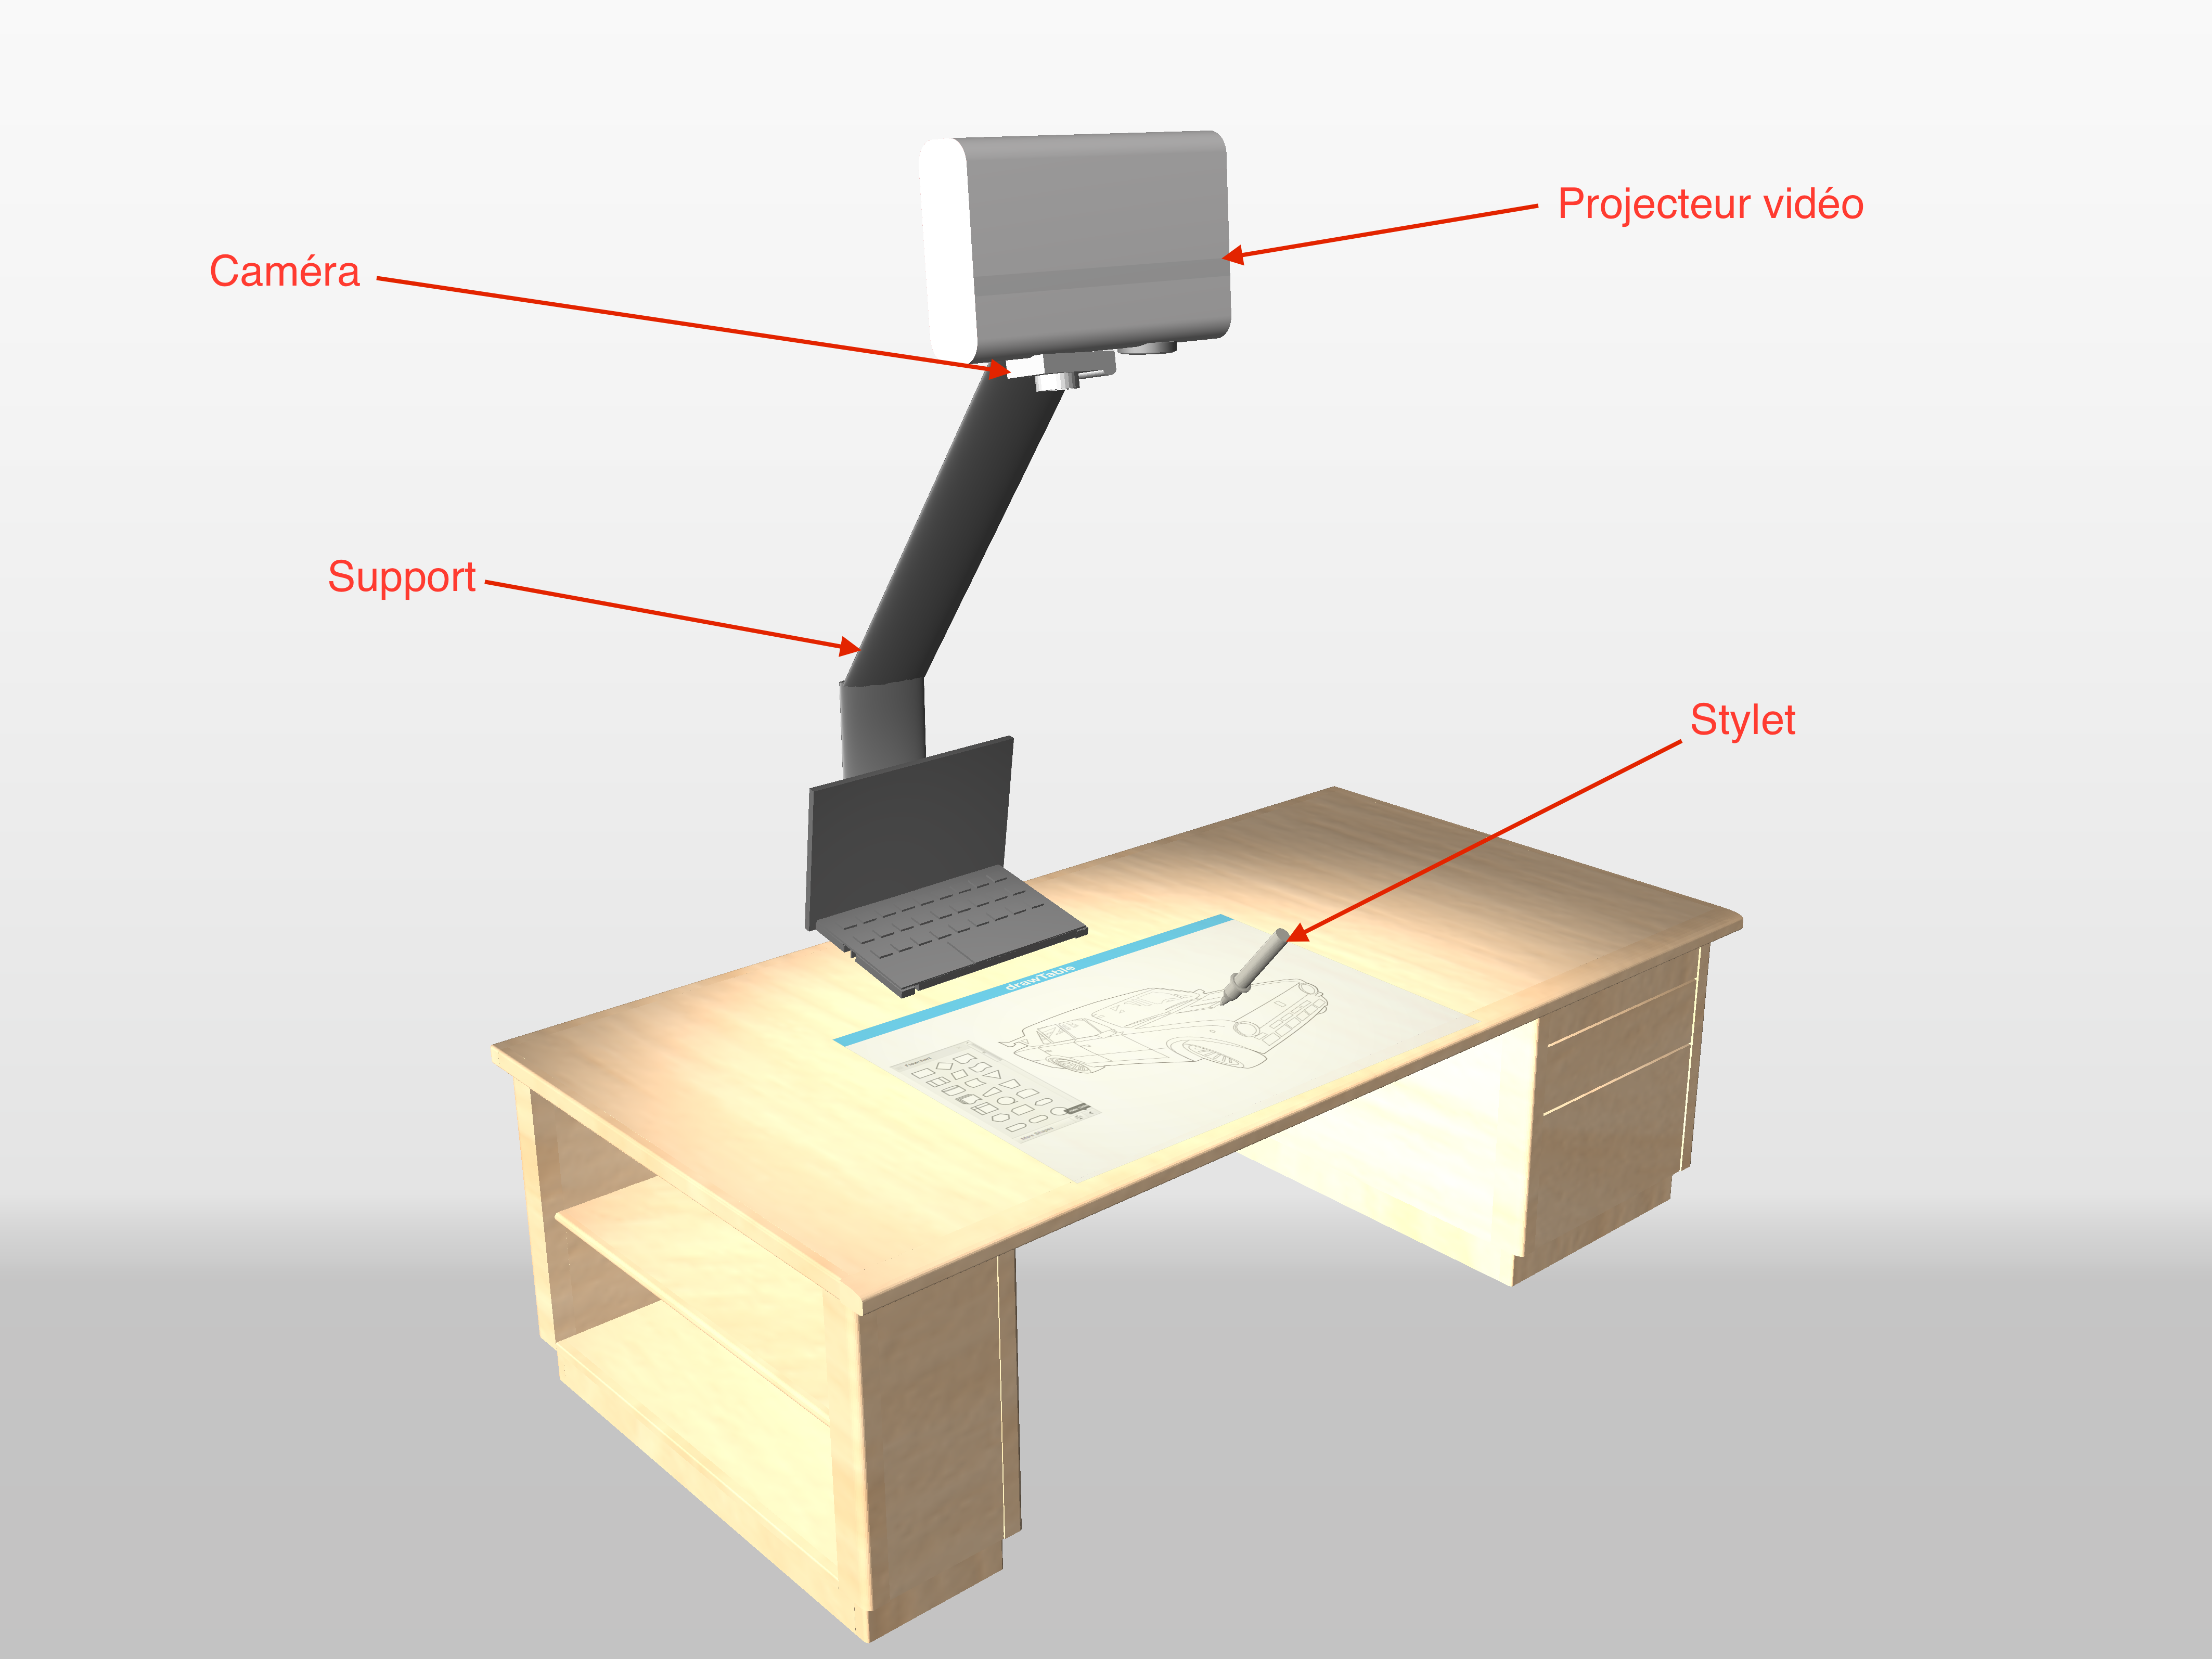
\includegraphics[scale=0.055]{images/drawing-environment.png}
\caption{Exemple d'environnement de dessin}
\end{figure}

\newpage

\section{Objectif du projet}

L'objectif de ce projet est de concevoir un outil de dessin assisté par ordinateur permettant à l'utilisateur de réaliser ses dessins de la manière la plus naturelle possible. À terme, l'utilisateur dessinera directement sur sa table ou n'importe quelle autre surface plane à l'aide d'un stylet et son dessin sera projeté sur son plan de travail, donnant ainsi à l'utilisateur l'impression de dessiner avec un crayon et une feuille.

\section{Technologies utilisées}

Les technologies utilisées pour le développement de l'application et le suivi du stylet sont les suivantes:

\begin{itemize}
\item[$\bullet$] Qt 5.5: Le framework Qt est une API orientée objet offrant des composants d'interface graphique, d'accès aux données, de connexions réseaux, de gestion des fils d'exécution, \dots. Dans le cadre du projet, elle est utilisée pour construire l'interface graphique utilisateur de l'application. Pour de plus amples informations, veuillez-vous référer au site officiel \url{http://www.qt.io}.
\item[$\bullet$] OpenCV 3.1: Open Computer Vision (OpenCV) est une bibliothèque graphique libre spécialisée dans le traitement d'images en temps réel. La bibliothèque OpenCV met à disposition de nombreuses fonctionnalités pour le traitement d'images, le traitement vidéos, les calculs matriciels, \dots. Dans le cadre du projet, elle est notamment utilisée pour le tracking du stylet. Pour de plus amples informations, veuillez-vous référer au site officiel \url{http://opencv.org}.
\item[$\bullet$] C++11: Le C++ est utilisé en guise de langage de programmation de base permettant de manipuler les différentes librairies utilisées dans le cadre du développement du projet. La librairie OpenCV et le framework Qt utilisant par défaut le langage C++, celui-ci constitue donc un choix idéal pour le développement du système.
\end{itemize}

\section{Équipe de projet}

Le tableau suivant présente l'équipe de projet, la hiérarchie au sein du groupe ainsi que les rôles joués par les différents membres du groupe:

\begin{table}[h]
\centering
\begin{tabular}{|l|l|c|l|}
\hline
\multicolumn{1}{|c|}{\textbf{Nom, prénom}} & \textbf{Hiérarchie}                 & \multicolumn{1}{c|}{\textbf{Rôles}} \\ \hline
Bron, Sacha                & \multicolumn{1}{l|}{Chef de projet} & Prototypes, gestion caméras, expérience utilisateur                                    \\ \hline
Villa, David               & \multicolumn{1}{l|}{Chef suppléant} & Interface graphique, outils de dessin                                    \\ \hline
Kammoun, Yassin            & -                                   & Interface graphique, documentation                                    \\ \hline
Ntawuruhunga, Paul         & -                                   & Tracking, calibrage, tests                                    \\ \hline
Pellet, Marc               & -                                   & Interface graphique, outils de dessin                                    \\ \hline
\end{tabular}
\caption{Équipe de projet}
\end{table}

\section{Cadre de réalisation}

Ce projet s'inscrit dans le cadre du cours de Projet de Groupe (PDG) au sein de la Haute École d'ingénierie et de gestion du canton de Vaud (HEIG-VD) sis à Yverdon-les-Bains. Selon le plan d'études de l'école, il est dispensé aux étudiants IL du département des Technologies de l'Information et de la Communication (TIC) pour le compte de leur troisième année de formation Bachelor. Le but de ce cours est d’effectuer un projet en passant par toutes les étapes de développement. Cela inclut le choix d'un sujet, la définition d’un cahier des charges, une phase de recherche et d'analyse suivie du développement de l’application et d’une phase de tests et de validation. En dernière instance, un rapport sur le déroulement du travail et une présentation du projet sont requis dans le but d'évaluer le travail effectué.

\section{Choix du sujet}

Le choix d'un tel sujet se justifie par le fait que ce projet exige un important travail de recherche, de découverte et d'apprentissage de nouvelles technologies comme cela peut notamment être le cas pour la librairie OpenCV. Bien évidemment, ce genre de projet présente des risques compte tenu du fait que la technologie n'est connue de personne, qu'elle peut être difficile à appréhender, à mettre en oeuvre et à maîtriser, que la faisabilité du projet n'est pas facilement définissable et que le temps d'apprentissage est difficilement estimable. Toutefois, toutes ces problématiques ne rendent le projet que plus motivant, attrayant et intéressant. 

Ce projet s'inscrivant dans un cadre académique, il s'agit donc d'une opportunité idéale d'acquérir de nouvelles connaissances. Le sujet en lui-même est des plus intéressants. Il se démarque clairement de la monotonie des applications développées dans un tel contexte. Des projets similaires ont certainement déjà été réalisés que ce soit dans un cadre professionnel que dans un cadre académique mais à bien moindre mesure ce qui laisse énormément de place pour la créativité et l'innovation. Par ailleurs, la complexité d'un tel projet ne rend que plus grand le mérite une fois le travail terminé avec un système tout à fait fonctionnel.

D'un point de vue organisationnel, ce projet présente la particularité d'être subdivisé en deux sous-projets étant donné que deux programmes sont développés: l'outil de dessin et le système de tracking du stylet. Un troisième sous-projet pourrait encore ressortir de ces deux derniers puisque la conception et la fabrication du stylet est un travail à part entière. Ainsi, un défi clairement établi de ce projet est l'intégration des différentes composantes pour finalement former un tout.

En dernière instance, ce sujet de projet a été choisi en premier lieu par son originalité puisque il s'avère fort différent des travaux réalisés dans le cadre de la formation Bachelor. Par ailleurs, le fait qu'il présente une difficulté certaine et un risque potentiel d'échec rend le projet d'autant plus motivant à réaliser. Enfin, l'étude d'une nouvelle technologie telle que la librairie OpenCV jusque-là parfaitement inconnue à l'équipe est attrayante puisqu'elle permet à chaque membre du groupe d'enrichir son bagage technique.

%----------------------------------------------------------------------------------------
%	CONCEPTION
%----------------------------------------------------------------------------------------

\chapter{Conception}

Ce chapitre se veut être une description complète aussi bien de la conception du système que de la conception du stylet. Il débute donc par la présentation complète du système. Cette présentation introduit dans un premier temps une vision globale du système. Cette étape préliminaire est suivie par une description détaillée et progressive de chaque composant du système. Il s'agit concrètement de présenter en fond et en large l'architecture de l'ensemble du système, de chaque sous-système et de leurs composants respectifs. Des diagrammes de classes et des diagrammes d'activités accompagnent cette description du système. Les différents modèles de stylet pour leur part sont introduits en premier lieu par une description de leur principe d'utilisation. Une présentation des différents composants matériels qui les constitue est ensuite réalisée. Un exposé de leur prototype est effectué au moyen de schémas. Les étapes de fabrication de ces modèles sont énumérées et commentées en long et large par la suite. Enfin, le fonctionnement de chacun des modèles est introduit. En dernière instance, l'environnement de dessin idéal est schématisé à l'aide de modélisations accompagnées de descriptions.

\section{Système global}

Cette section présente l'ensemble du système d'un point de vue global. Le but est d'être aussi abstrait que possible de manière à ce que l'étude du système se fasse de manière progressive. Cette présentation débute par l'introduction de l'architecture du système. 

Le système global correspond en la réunion de l'infrastructure matérielle et des composants logiciels compte tenu de la nature du projet. Cela se justifie notamment par le fait que des composants matériels interagissent avec des composants logiciels et inversement.

\subsection{Architecture}

L'architecture est présentée en deux variantes: une vue d'ensemble et une vue détaillée. Cette dernière n'est là qu'à titre indicatif de façon à ce que le lecteur dispose de la version complète de l'architecture; elle ne fait pas l'objet d'une description, seule la version allégée le fait.

\newpage

\subsubsection{Vue d'ensemble}

La figure suivante propose une vue d'ensemble de l'architecture de du système dans sa globalité:

\begin{figure}[H]
\centering
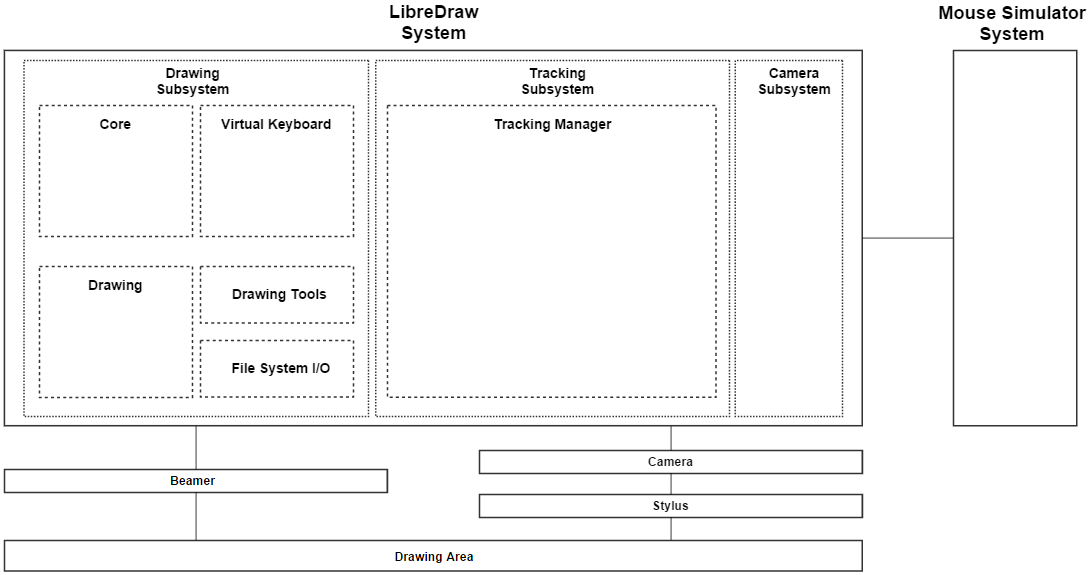
\includegraphics[angle=90, scale=0.75]{overview-global-system-architecture.png}
\caption{Vue d'ensemble de l'architecture du système global}
\end{figure}

Le système dans sa globalité est en fait constitué de deux systèmes à part entière qui sont respectivement \textbf{LibreDraw System} et \textbf{Mouse Simulator System}. Par ailleurs, le système global est caractérisé par des éléments externes d'ordre matériel interagissant avec les deux systèmes mentionnés plus tôt; il s'agit concrètement des éléments \textit{Beamer}, \textit{Camera}, \textit{Stylus} et \textit{Drawing Area}.

Le système \textbf{LibreDraw System} correspond à l'application de dessin à proprement parlé laquelle gère aussi bien la partie outil de dessin que la partie tracking du stylet. Ces tâches sont gérées respectivement par les sous-systèmes \textbf{Drawing Subsystem} et \textbf{Tracking Subsystem}. Par ailleurs, ce même système est caractérisé par un sous-système supplémentaire à savoir \textbf{Camera Subsystem}. Celui-ci a pour objectif de gérer l'initialisation et la mise à jour de la communication avec un dispositif d'enregistrement vidéo, une caméra donc, connecté au système hôte. Autrement dit, il s'agit de l'élément matériel \textit{Camera}.

Le sous-système \textbf{Drawing Subsystem} contient entre autres le \textit{Core} de l'application du point de vue expérience utilisateur, c'est-à-dire son interface graphique. Par ailleurs, compte tenu du fait que l'interaction de ce même utilisateur avec l'application s'effectue par le biais d'un stylet, un clavier virtuel est mis à disposition par le constituant \textit{Virtual Keyboard} pour toute saisie textuelle d'information. L'esquisse du dessin de l'utilisateur avec le stylet est reproduite par le constituant \textit{Drawing}. Cette reproduction est appliquée par des outils de dessin regroupés dans le constituant \textit{Drawing Tools}. La sérialisation d'un dessin, sa sauvegarde et son importation au sein de l'application, est rendue possible par la mise à disposition de fonctionnalités fournies par le constituant \textit{File System I/O}.

Le sous-système \textbf{Tracking Subsystem} est caractérisé par un constituant unique; il s'agit du \textit{Tracking Manager}, le gestionnaire du suivi du stylet dit autrement. En plus de gérer le stylet, ce constituant assure l'initialisation et la configuration de l'ensemble de l'infrastructure du système: écran, caméra et stylet. 

Le système \textbf{Mouse Simulator System} est un composant à part entière. Celui-ci permet comme son nom l'indique de simuler une souris, c'est-à-dire de reproduire les faits et gestes de l'utilisateur lors de la manipulation du stylet comme s'il utilisait une souris en lieu et place de ce même stylet. 

Le système dans son ensemble fonctionne globalement de la manière suivante:

\begin{enumerate}
\item Le lancement de l'application débute par l'initialisation et la configuration de l'infrastructure système. Ceci est réalisé par le constituant \textit{Tracking Manager} du sous-système \textbf{Tracking Subsystem}.
\item Une fois la phase de configuration et d'initialisation terminée, les éléments matériels \textit{Camera} et \textit{Stylus} sont opérationnels et exploitables.
\item L'interaction de l'utilisateur par le stylet avec l'application est capturée par l'élément \textit{Caméra} qui communique l'information au constituant \textit{Tracking Subsystem}.
\item L'analyse des faits et gestes de l'utilisateur par le constituant \textit{Tracking Manager} est communiquée au système \textbf{Mouse Simulator System}. Celui-ci simule l'action utilisateur et l'applique sur le sous-système \textbf{Drawing Subsystem} du système \textbf{LibreDraw}.
\item Le constituant \textit{Drawing} du sous-système \textbf{Drawing Subsystem} veille à reproduire l'esquisse de l'utilisateur. Un élément adéquat du constituant \textit{Drawing Tools} est utilisé pour ce faire.
\item L'élément matériel \textit{Beamer} veillera à projeter la reproduction du dessin de l'utilisateur réalisé par l'élément \textit{Stylus} sur le support de dessin physique représenté par l'élément \textit{Drawing Area}.
\end{enumerate}

\newpage

\subsubsection{Vue détaillée}

La figure suivante propose une vue détaillée de l'architecture de du système dans sa globalité:

\begin{figure}[H]
\centering
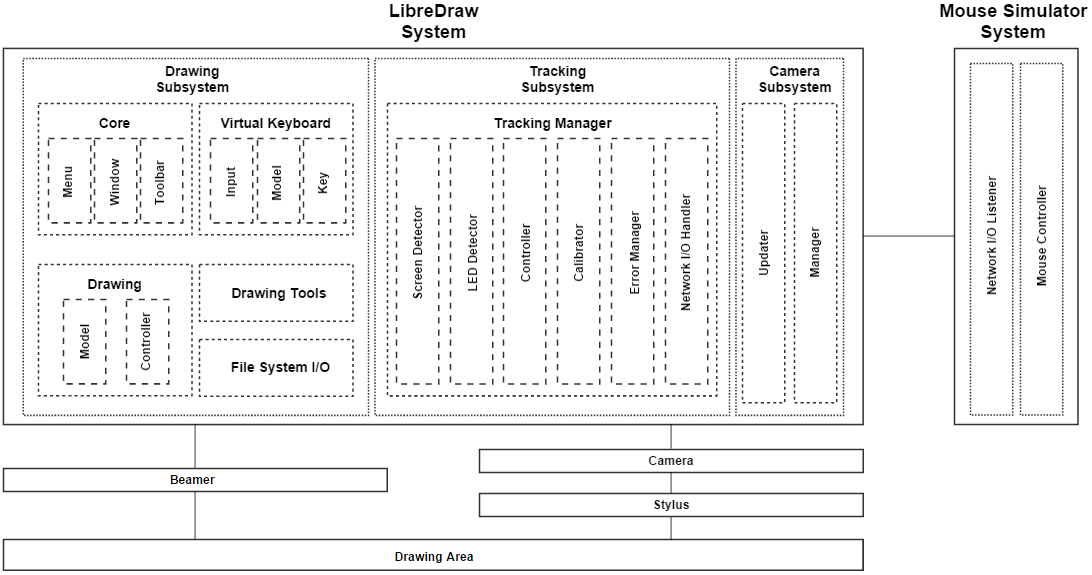
\includegraphics[angle=90, scale=0.75]{detailled-global-system-architecture.png}
\caption{Vue détaillée de l'architecture du système global}
\end{figure}

\newpage

\subsection{Diagramme d'activités}

La figure suivante illustre l'activité globale liée à une esquisse utilisateur réalisée au moyen du stylet:

\begin{figure}[H]
\centering
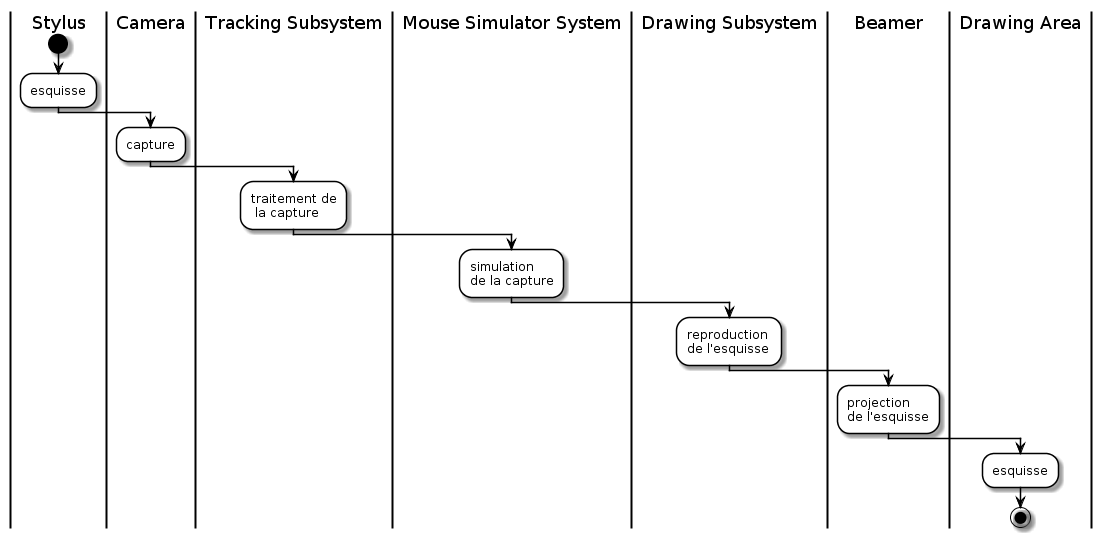
\includegraphics[angle=90, scale=0.55]{global-drawing-activity.png}
\caption{Activité globale d'une esquisse utilisateur}
\end{figure}

\subsection{Diagramme de classes}

\subsubsection{Vue d'ensemble}

\subsubsection{Vue détaillée}

\newpage

\section{LibreDraw System}

Cette section présente le détail de la conception du système \textbf{LibreDraw System}. Cette présentation débute par l'introduction de l'architecture de ce système. Celle-ci est bien plus détaillée de manière à approfondir progressivement la description du système. Chaque constituant du système fait également l'objet d'une pareille décomposition et d'une pareille description. Ce système correspond à l'application de dessin à proprement parlé. Pour rappel, l'application se veut être un outil de dessin assisté par ordinateur permettant à l'utilisateur de réaliser ses dessins de la manière la plus naturelle possible. Il doit pouvoir dessiner directement sur sa table ou n'importe quelle autre surface plane à l'aide d'un stylet. Son dessin doit pour sa part être projeté sur son plan de travail, donnant à l'utilisateur l'impression de dessiner avec un crayon et une feuille. Une telle application nécessite bien évidemment la mise en place d'une infrastructure adéquate. Toutefois, cette infrastructure doit pouvoir être exploitée par l'application. 

Le mécanisme de suivi du stylet étant relativement complexe, il ne peut en aucune manière être exécuté sans passer au préalable par une phase d'initialisation et de configuration. En effet, différents objectifs doivent être atteints initialement de manière à ce que le système de tracking soit non seulement en mesure d'interagir avec le matériel mais en plus, que son interaction s'effectue de la manière la plus optimale possible. Le système doit être capable de s'adapter à un certain nombre de contraintes. Celles-ci peuvent être d'ordre matériel. En effet, malgré la présence conseillée d'une caméra et d'un projecteur, il n'en demeure pas moins qu'elle n'est pas obligatoire. En conséquence, l'application doit être en mesure de s'adapter lors d'une telle situation. Par ailleurs, le fait de disposer d'une caméra connectée au système hôte n'est pas suffisant pour que le système de tracking soit en mesure d'interagir de manière performante avec l'ensemble de l'infrastructure. L'angle et la position de la caméra étant des informations tout à fait variables, elles doivent être prises en compte lors de l'initialisation du mécanisme de tracking.

Le suivi du stylet n'est également pas une tâche facile. Le mécanisme de tracking doit être en mesure de détecter à tout moment le stylet tant qu'il reste dans le champ de vision de la caméra et ce, indépendamment de la gestuelle de l'utilisateur. Le principe de détection de stylet défini lors de l'établissement du cahier des charges reposant sur la détection de LED, celui-ci découle à un certain nombre de problèmes potentiels et de questions devant être imaginées, supposées et répondues à l'avance. Une de ces questions est le comportement du mécanisme de tracking lorsque la LED du stylet présente la même couleur que le contenu du dessin de l'utilisateur. Ainsi, le dessin et la LED risqueraient d'être confondues. Telles sont les problématiques auxquelles le système de tracking doit faire face. L'ergonomie de l'application et l'expérience utilisateurs sont tout autant des points à soulever. L'interaction de l'utilisateur avec l'application s'effectuant avec un stylet, celle-ci peut être sujette à des problèmes de précision. Par ailleurs, les situations de saisies d'information par l'utilisateur doivent être rendues aussi facile que possible. En effet, forcer l'utilisateur a quitté son support de travail pour être en mesure de sauvegarder son dessin par le biais de son clavier physique est une contrainte qui est loin d'être appréciable. De ce fait, une solution permettant à l'utilisateur d'accomplir une telle tâche en se passant de son clavier doit être proposée. Le fait que les faits et gestes de l'utilisateur soient captés par une caméra vidéo et interprétés nécessite de reproduire l'esquisse de dessin déclenchée par l'utilisateur dans l'application de dessin. Le dessin esquissé par l'utilisateur étant projeté via un projecteur sur son support de travail, le dessin doit donc être reproduit logiquement et visuellement au sein de l'application.

\newpage

\subsection{Architecture}

La figure suivante illustre l'architecture du système \textbf{LibreDraw System}:

\begin{figure}[H]
\centering
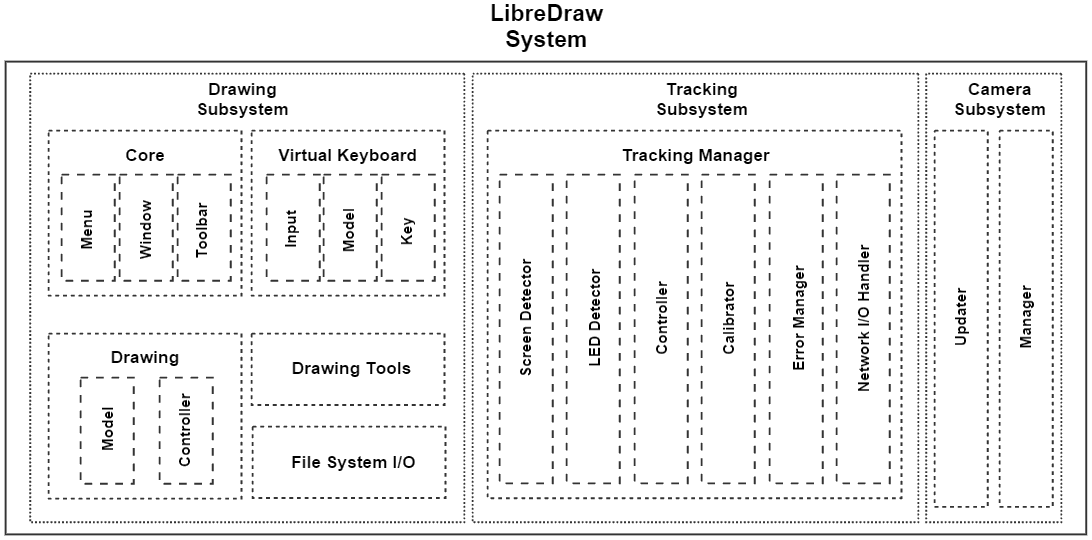
\includegraphics[angle=90, scale=0.75]{libredraw-system-architecture.png}
\caption{Architecture du système LibreDraw System}
\end{figure}

Le système \textbf{LibreDraw System} est divisé en trois sous-systèmes distincts. Le premier sous-système est \textbf{Camera Subsystem}. Celui-ci a pour tâches de gérer l'initialisation, la configuration et sélection de la caméra utilisateur devant servir à capturer les mouvements du stylet. La partie initialisation et configuration est assurée par le constituant \textit{Manager}. Celui-ci fait appel au constituant \textit{Updater} pour proposer une liste de caméras disponibles susceptibles d'être utilisées en guires de dispositif d'enregistrement vidéo de l'application.

Le second sous-système du système \textbf{LibreDraw System} est \textbf{Tracking Manager}. Celui-ci est constitué d'un constituant principal qui est le gestionnaire du tracking de stylet. Il a pour tâche principale, comme son nom l'indique, de gérer le tracking du stylet, c'est-à-dire d'assurer en permanence son suivi au sein du champ de vision de la caméra.

Le dernier sous-système du système \textbf{LibreDraw System} est \textbf{Drawing Subsystem}. Celui-ci gère entre autres toute la partie interface graphique utilisateur de l'application de dessin. Il dispose en premier lieu d'un constituant nommé \textit{Core} qui fait office de coeur de l'interface. Il met également à disposition un constituant \textit{Virtual Keyboard} qui fournit comme son nom l'indique un clavier virtuel. Celui-ci est sollicité entre autres lors de chaque saisie utilisateur. 

Le dessin de l'utilisateur est représenté pour sa part par le constituant \textit{Drawing}. Ce dernier gère toute la partie reproduction de dessin aussi bien au niveau logique que graphique. Il délègue toutefois l'application de l'esquisse réalisée à l'aide d'un outil à des éléments du constituant \textit{Drawing Tools}. Finalement, le dernier constituant composant ce sous-système est \textit{File System I/O} qui met à disposition des mécanismes de sérialisation de dessin.

\newpage

\subsection{Diagramme d'activités}

\subsection{Diagramme de classes}

\newpage

\subsection{Drawing Subsystem}

Cette section présente le détail de la conception du sous-système \textbf{Drawing Subsystem} du système \textbf{LibreDraw System}. Cette section présente le détail de la conception du sous-système \textbf{Drawing Subsystem}. Cette présentation débute par l'introduction de l'architecture de ce système. Celle-ci est bien plus détaillée de manière à approfondir progressivement la description du système. Chaque constituant du système fait également l'objet d'une pareille décomposition et d'une pareille description.

L'interface graphique utilisateur doit concrètement proposer une fenêtre principale dans laquelle il est possible de dessiner. Bien évidemment, il est attendu de l'utilisateur qu'il dessine à l'aide du stylet sur son support de travail. Toutefois, il ne lui est pas impossible de travailler directement sur l'application au moyen de la souris de son ordinateur. Ce n'est évidemment pas jouir de la fonctionnalité principale de l'application de dessin. Néanmoins, aucune contrainte de cet ordre n'est imposée à l'utilisateur quant à l'esquisse de son dessin.

L'esquisse d'un dessin doit pouvoir être effectuée dans une zone appropriée laquelle correspond en un espace ouvert où l'utilisateur peut esquisser ce qu'il désire et ce, à sa guise. Par ailleurs, il doit disposer d'une panoplie d'outils lui permettant d'être inventif et créatif vis-à-vis de son dessin tant sur sa forme que sur son contenu. Les points suivants récapitulent les outils devant être mis à disposition:

\begin{itemize}
\item[$\bullet$] Outils de dessin: les outils de dessin mettent à disposition un crayon et une gomme permettant de dessiner sans restriction n'importe quelle forme géométrique.
\item[$\bullet$] Outils de formes: les outils de formes mettent à disposition un ensemble de formes géométriques prédéfinies pouvant être dessinées au sein d'un dessin et redimensionnées à la guise de l'utilisateur.
\item[$\bullet$] Outils de couleurs: les outils de couleurs mettent à disposition une palette de couleurs laquelle permet de définir la couleur du trait aussi bien pour les outils de dessin que pour les outils de formes.
\item[$\bullet$] Outils d'épaisseur: les outils d'épaisseur permettent de définir selon une liste prédéfinie l'épaisseur du trait aussi bien pour les outils de dessin que pour les outils de formes.
\end{itemize}

Le dessin esquissé par l'utilisateur doit pouvoir être sauvegardé de manière à pouvoir y retravailler dessus ultérieurement. De ce fait, des boîtes de dialogue adaptées à l'utilisation d'un stylet doivent être proposées de manière à pouvoir effectuer de telles opérations. De plus, ces boîtes de dialogue doivent permettre l'utilisateur d'y saisir aisément du texte. En conséquence, une solution de saisie doit être proposée et celle-ci doit être en adéquation avec l'utilisation d'un stylet lors de l'accomplissement d'une telle tâche.

En dernière instance, l'interface graphique utilisateur doit être ergonomique, facile d'utilisation et agréable à l'utilisateur. Le point essentiel est l'aisance avec laquelle il doit être en mesure d'interagir avec l'interface graphique de l'application en recourant au stylet. En conséquence, l'élaboration de toutes les fenêtres, boîtes de dialogues et autres doivent impérativement être imaginées de telle sorte que l'utilisation du stylet remplace définitivement celle de la souris de l'ordinateur.

\newpage

\subsubsection{Architecture}

La figure suivante illustre l'architecture du sous-système \textbf{Drawing Subsystem}:

\begin{figure}[H]
\centering
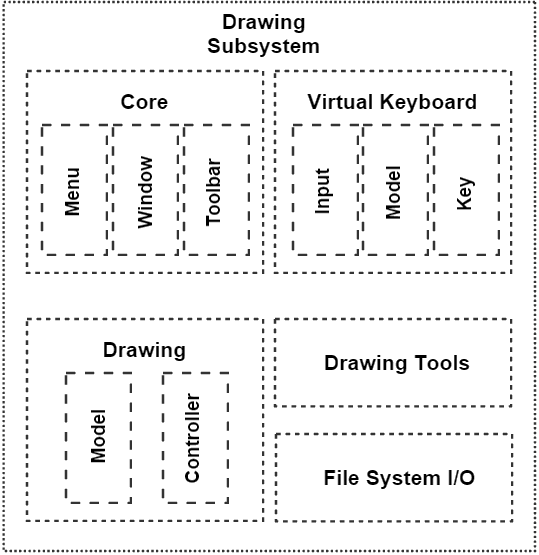
\includegraphics[scale=0.9]{drawing-subsystem-architecture.png}
\caption{Architecture du sous-système Drawing Subsystem}
\end{figure}

Le sous-système \textbf{Drawing Subsystem} gère entre autres toute la partie interface graphique utilisateur de l'application de dessin. Le composant \textit{Core} correspond au coeur de ce sous-système et donc, à l'interface graphique de l'application. Celui-ci met effectivement à disposition tous les constituants graphiques nécessaires devant être combinés et regroupés ensemble pour former finalement l'interface utilisateur final. Il s'agit concrètement des constituants \textit{Menu} qui fournit le menu de l'application de dessin, \textit{Window} qui correspond à la fenêtre principale de l'application et enfin, \textit{Toolbar} qui se révèle être la barre d'outils de cette même fenêtre.

La sérialisation d'un dessin est rendue possible par le constituant \textit{File System I/O} qui fournit deux boîtes de dialogue permettant respectivement d'importer et de sauvegarder un dessin. La problématique liée à la saisie utilisateur par le biais du stylet est répondue grâce au constituant \textit{Visual Keyboard}. Ce dernier fournit un clavier virtuel s'apparentant aux claviers usuels que l'on rencontre sur les applications des smartphones et des tablettes. Ainsi, les boîtes de dialogue mentionnées plus tôt intègrent ce clavier dans leur interface. 

Les constituants \textit{Drawing} et \textit{Drawing Tools} collaborent ensemble en vue de produire le dessin esquissé par l'utilisateur. Pour ce faire, un élément \textit{Controller} veille à appliquer l'esquisse sur le \textit{Model} du dessin en prenant en compte l'outil courant proposé par le constituant \textit{Drawing Tools}. À noter que, durant la totalité de son interaction avec l'interface graphique, l'utilisateur peut à tout moment recourir à la souris de son ordinateur pour réaliser les mêmes traitements qu'il était supposé réalisé initialement par le biais du stylet. Ainsi, la possibilité de s'abstenir d'utiliser le stylet demeure toujours possible pour l'utilisateur.

En définitive, le sous-système \textbf{Drawing Subsystem} fait collaborer l'ensemble de ses composants en vue de reproduire le dessin esquissé par l'utilisateur et de sérialiser ce dessin en recourant au clavier virtuel fournit par \textit{Visual Keyboard}. Ce dernier se révèle être en parfaite adéquation avec une saisie utilisateur au moyen d'un stylet.

\subsubsection{Core}

Cette sous-section décrit le composant \textit{Core}. Il s'agit de présenter son architecture, de la décomposer pour ensuite introduire individuellement ses constituants.

Le composant \textit{Core} correspond en l'interface graphique de la fenêtre principale de l'application.

\textbf{Architecture}

La figure suivante illustre l'architecture du composant \textit{Core} du sous-système \textbf{Drawing Subsystem}:

\begin{figure}[H]
\centering
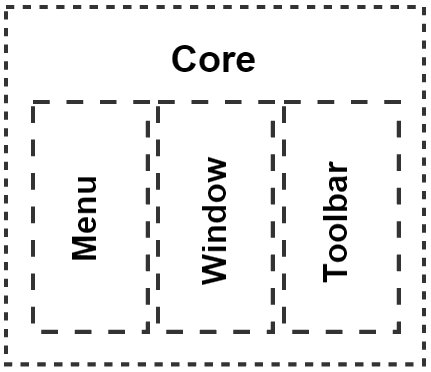
\includegraphics[scale=0.9]{core-component-architecture.png}
\caption{Architecture du composant Core}
\end{figure}

Le composant \textit{Core} a pour base l'élément \textit{Window} qui consiste en la fenêtre principale de l'application. Dans cette fenêtre figure l'élément \textit{Toolbar} faisant office de barre d'outils de la fenêtre. Cette barre d'outils permet de sélectionner un outil de dessin, de forme ou d'exécuter l'outil d'épaisseur, les outils d'historique des actions ou encore l'outil palette de couleurs. Par ailleurs, cette même barre permet d'accéder au menu de l'application représenté par l'élément \textit{Menu}.

\textbf{Window}

La figure suivante illustre la structure de l'élément \textit{Window}:

\begin{figure}[H]
\centering
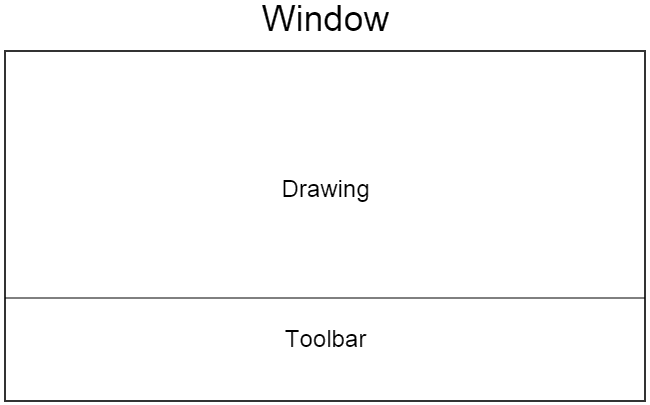
\includegraphics[scale=0.9]{window-element-structure.png}
\caption{Structure de l'élément Window}
\end{figure}

L'élément \textit{Window} est composé d'une part par le composant \textit{Drawing} censé contrôlé et stocké le desin de l'utilisateur. D'autre part, il est caractérisé par l'élément \textit{Toolbar} laquelle met à disposition un ensemble d'outils susceptibles de contribuer à l'esquisse du dessin, à modifier certaines propriétés de l'élément \textit{Controller} du composant \textit{Drawing} comme l'épaisseur du trait. Par ailleurs, ce même élément \textit{Toolbar} permet d'accéder à l'élément \textit{Menu}.

\textbf{Menu}

La figure suivante illustre la structure de l'élément \textit{Menu}:

\begin{figure}[H]
\centering
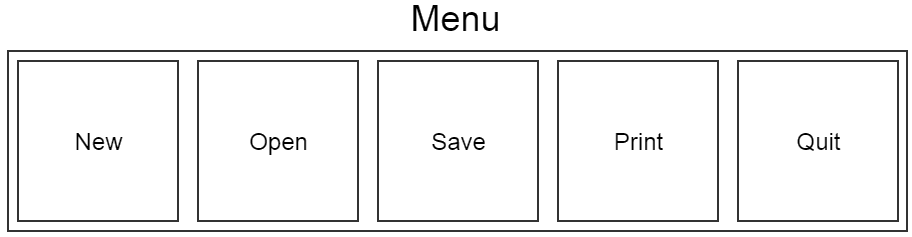
\includegraphics[scale=0.9]{menu-element-structure.png}
\caption{Structure de l'élément Menu}
\end{figure}

L'élément \textit{Menu} est accessible via l'élément \textit{Window} par le déclenchement d'un outil adéquat de l'élément \textit{Toolbar}. Cet élément \textit{Menu} est composé pour sa part par des boutons lesquels permettent d'exécuter des fonctionnalités données liées à la manipulation usuelle d'un document comme sa création, sa sauvegarde et autres.

\textbf{Toolbar}

La figure suivante illustre la structure de l'élément \textit{Toolbar}:

\begin{figure}[H]
\centering
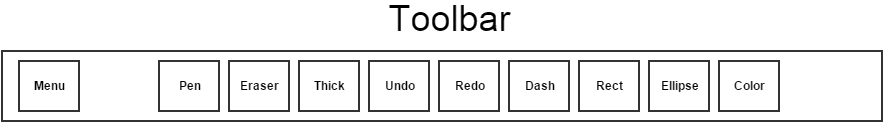
\includegraphics[scale=0.9]{toolbar-element-structure.png}
\caption{Structure de l'élément Toolbar}
\end{figure}

L'élément \textit{Toolbar} est constitué d'un ensemble de boutons. Un premier bouton s'écarte toutefois du lot; il s'agit du bouton avec pour label "Menu". Celui-ci permet évidemment d'ouvrir l'élément \textit{Menu} de la fenêtre. Le reste des autres boutons est à part. Certains d'entre eux permettent d'esquisser des formes géométriques ou de dessiner à main levée. D'autres permettent de personnaliser les traits tant au niveau de la couleur que de l'épaisseur. Enfin, certains permettent d'agir sur l'historique des actions, annuler ou rétablir une action autrement dit.

\subsubsection{Virtual Keyboard}

Cette sous-section décrit le composant \textit{Virtual Keyboard}. Il s'agit de présenter son architecture, de la décomposer pour ensuite introduire individuellement ses constituants.

Le composant \textit{Virtual Keyboard} correspond en un clavier virtuel lequel permet à l'utilisateur de saisir des informations au sein par le biais du stylet.

\textbf{Architecture}

La figure suivante illustre l'architecture du composant \textit{Virtual Keyboard} du sous-système \textbf{Drawing Subsystem}:

\begin{figure}[H]
\centering
\includegraphics[scale=0.9]{keyboard-component-structure.png}
\caption{Architecture du composant Virtual Keyboard}
\end{figure}

Le composant \textit{Virtual Keyboard} est caractérisé avant tout par un élément \textit{Model}, correspondant au modèle du clavier, c'est-à-dire à la disposition de ses touches. Chacune des touches du clavier correspondent pour leur part à des éléments \textit{Key}. L'élément \textit{Input} consiste en ce qui le concerne en un champ texte éditable lequel est lié à un clavier virtuel. Autrement dit, la saisie de texte dans ce champ n'est possible que par le composant \textit{Virtual Keyboard} qui lui aurait été associé.

\textbf{Model}

L'élément \textit{Model} correspond pour le composant \textit{Virtual Keyboard} la disposition de ses touches représentés par des éléments \textit{Key}.

Les figures suivantes illustrent l'agencement des touches du clavier:

\begin{figure}[H]
\centering
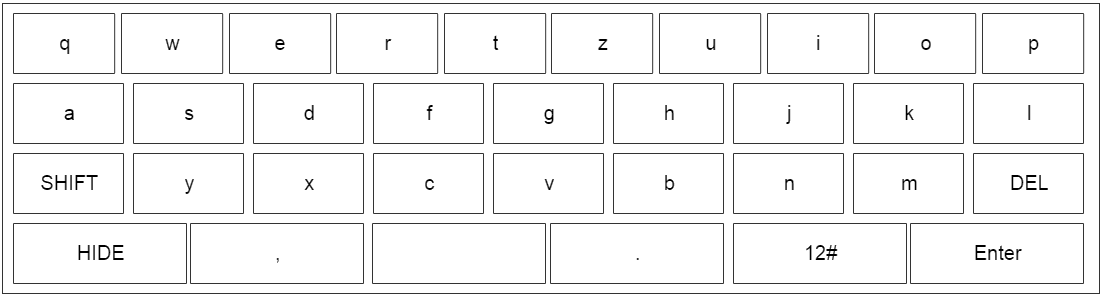
\includegraphics[scale=0.9]{keyboard-layout-letter.png}
\caption{Agencement des touches du clavier virtuel selon le mode lettre}
\end{figure}

\begin{figure}[H]
\centering
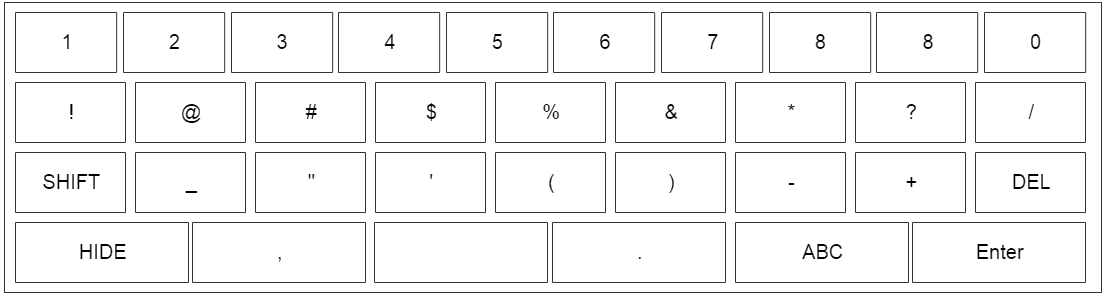
\includegraphics[scale=0.9]{keyboard-layout-symbol.png}
\caption{Agencement des touches du clavier virtuel selon le mode symbole}
\end{figure}

\textbf{Key}

L'élément \textit{Key} représente une touche du clavier virtuel représenté par le composant \textit{Virtual Keyboard}. Ce dernier faisant l'objet de deux agencements, certains de ses éléments \textit{Key} sont amenés à changer de valeur. Ainsi, on dénombre deux modes différents pour un élément \textit{Key}:

\begin{itemize}
\item[$\bullet$] Le mode mono-évalué: en mode symbole ou en mode lettre, la même valeur est retournée.
\item[$\bullet$] Le mode multi-évalué: en mode symbole ou en mode lettre, une valeur différente est retournée.
\end{itemize}

Les figures suivantes illustrent les deux formes possibles que peut prendre un élément \textit{Key}:

\begin{figure}[H]
\centering
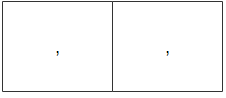
\includegraphics[scale=0.9]{keyboard-key-mono.png}
\caption{Elément Key mono-evalué}
\end{figure}

\begin{figure}[H]
\centering
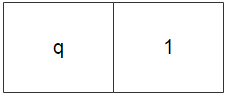
\includegraphics[scale=0.9]{keyboard-key-multi.png}
\caption{Elément Key multi-evalué}
\end{figure}

\textbf{Input}

L'élément \textit{Input} correspond en un champ texte éditable uniquement par le biais d'un composant \textit{Virtual Keyboard}. Ainsi, lors du focus sur ce champ texte, le clavier virtuel est aussitôt affiché.

\subsubsection{Drawing}

Cette sous-section décrit le composant \textit{Drawing}. Il s'agit de présenter son architecture, de la décomposer pour ensuite introduire individuellement ses constituants.

Le composant \textit{Drawing} correspond au dessin de l'utilisateur.

\textbf{Architecture}

La figure suivante illustre l'architecture du composant \textit{Drawing} du sous-système \textbf{Drawing Subsystem}:

\begin{figure}[H]
\centering
\includegraphics[scale=0.9]{drawing-component-structure.png}
\caption{Architecture du composant Drawing}
\end{figure}

Le composant \textit{Drawing} est composé d'un élément \textit{Model} qui représente le dessin aussi bien logiquement que visuellement. Ce composant est également caractérisé par l'élément \textit{Controller}. Celui-ci assure la reproduction des esquisses de l'utilisateur sur demande du système \textbf{Mouse Simulator System}.

\textbf{Model}

L'élément \textit{Model} représente le dessin de manière logique et graphique. Il se repose sur une structure de type \textit{bitmap}, c’est-à-dire une matrice où chaque élément correspond à un pixel. La valeur stockée dans un tel élément correspond à une couleur. Cette couleur est représentée quant à elle par un code hexadécimal. En guise d’exemple, la figure suivante illustre une telle structure.

\begin{figure}[H]
\centering
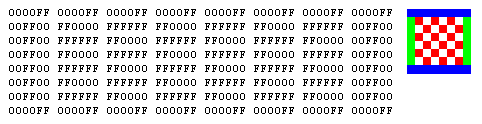
\includegraphics[scale=0.9]{drawing-structure.png}
\caption{Structure logique d’un dessin}
\end{figure}

\textbf{Controller}

L'élément \textit{Controller} veille à la bonne reproduction des esquisses de l'utilisateur lorsqu'il est sollicité par le système \textbf{Mouse Simulator System}. Il délègue la reproduction de l'esquisse à un élément du composant \textit{Drawing Tools}.

\subsubsection{Drawing Tools}

Le composant \textit{Drawing} correspond en un ensemble d'éléments associant aux outils accessibles via le composant \textit{Core} un contrôleur respectif. Ce contrôleur reproduit le geste de l'utilisateur selon l'outil sélectionné au moment donné. Il est à noter toutefois que cette association ne concerne que les outils susceptibles d'ajouter du contenu au dessin, esquisser à main levée ou esquisser des formes géométriques autrement dit.

\subsubsection{File System I/O}

Le composant \textit{File System I/O} met à disposition de l'application, et de l'utilisateur dans une moindre mesure, des mécanismes de sérialisation de dessin. Ceux-ci sont rendus accessibles à l'utilisateur par des interfaces graphiques se présentant sous la forme de boîtes de dialogue. Compte tenu du fait que ces boîtes de dialogue attendent de l'utilisateur de la saisie textuelle, les interfaces en question intègrent le composant \textit{Virtual Keyboard} lequel fournit un clavier virtuel permettant l'édition de champ texte et ce, en recourant au stylet.

\newpage

\subsection{Tracking Subsystem}

Le sous-système \textbf{Tracking Subsystem} est un composant essentiel de l'application ayant pour but de gérer le pointeur de l'utilisateur. En effet, étant donné que ce type de pointeur n'est pas une entrée standard comme pourrait l'être une souris ou un clavier, l'application a besoin d'un module prenant en charge exclusivement le suivi du stylet.

Ce module doit fournir une abstraction suffisante au \textbf{Drawing Subsystem} afin que les modules aient un minimum de dépendance et donc, que l'évolution d'un module n'influence pas l'autre.

\subsubsection{Architecture}

Les composants de ce sous-système peuvent être classé du niveau le plus bas au plus élevé:

\begin{itemize}
\item[$\bullet$] \textit{Calibrator}: ce constituant initialise et calibre l'infrastructure matériel de manière à ce qu'il puisse interagir avec l'application et inversement.
\item[$\bullet$] \textit{LED Detector}: ce constituant a pour fonction de détecter et traquer en permanence la/les LED(s) du stylet de manière à le localiser dans le champ de vision de la caméra. Cela est utilisé aussi bien lors de la phase d'initialisation du système que lors de sa phase post-initialisation, c'est-à-dire lors du suivi du stylet.
\item[$\bullet$] \textit{Screen Detector}: ce constituant a pour fonction de détecter l'écran de l'utilisateur. Cela est notamment utilisé lors de la phase préliminaire de calibrage du matériel. Il permet de décrire la position de la LED dans le référentiel de l'écran.
\item[$\bullet$] \textit{Error Manager}: ce constituant fait office de gestionnaire d'erreur. Il est notamment sollicité lors d'une erreur rencontrée durant le processus de calibrage.
\item[$\bullet$] \textit{Controller}: ce constituant contrôle les mouvements et les actions du stylet selon les informations reçues par la caméra et selon leur analyse également.
\item[$\bullet$] \textit{Network I/O Handler}: ce constituant fait office d'interface de communication réseau entre les systèmes \textbf{LibreDraw System} et \textbf{Mouse Simulator System}. Il est notamment sollicité une fois le traitement d'informations liés aux faits et gestes du stylet terminé afin de les reproduire au sein de la partie dessin du système gérée entre autres par le sous-système \textbf{Drawing Subsystem}.
\end{itemize}

Comme nous pouvons le voir, une fois que le calibrage est effectué, la caméra pourra détecter la LED du stylet. Ensuite, cette position sera transformée pour que l'on connaisse sa position par rapport à l'image du vidéo-projecteur (donc du programme) et sera ensuite utilisée pour envoyer des événements de mouvement de souris via le réseau.

\subsubsection{Controller}

\subsubsection{Screen Detector}

Le \textbf{Screen Detector} est un composant permettant de détecter l'écran vu depuis la caméra et d'en calculer les déformations par rapport à l'image qu'affiche le vidéo-projecteur. En effet, le pointeur de l'utilisateur se déplace dans le monde réel en trois dimensions, mais la caméra ne voit qu'une projection bidimensionnelle de ce monde et le projecteur envoie une image également bidimensionnelle. Dans le cas ou la caméra et le projecteur était exactement aligné, ils auraient la même perception du monde et aucun calcul ne serait nécessaire. Or, ce n'est pas le cas: la caméra peut se trouver plusieurs dizaines de centimètres à côté du projecteur. Ainsi, une matrice de transformation permettant de passer d'un référentiel à l'autre doit être calculé par le programme. En termes plus mathématiques, cette matrice nous permet d'effectuer une rotation tridimensionnelle, un déplacement et une mise à l'échelle de l'image afin de reporter les points du référentiel de la caméra à celui du programme.

\subsubsection{LED Detector}

Ce composant gère le suivi de la LED. Il peut être considéré comme bas niveau dans le sens qu'il s'occupe de traiter les données brutes venant directement de la caméra. Il y a donc plusieurs traitements à effectuer sur les images afin d'en faire ressortir le peu d'information utile, c'est-à-dire une position bidimensionnelle dans le référentiel de la caméra. Ces traitements ont été une partie très importante de ce travail car ils demandent beaucoup de tests dans des conditions différentes, ainsi que de l'imagination pour trouver la meilleure méthodologie à appliquer. Du temps a aussi été nécessaire pour trouver les paramètres les plus optimaux de nos filtres. Certains paramètres sont d'ailleurs fixes alors que d'autres sont calculés durant la phase de calibration.

\subsubsection{Calibrator}

Cette partie du programme s'occupe de calibrer le suivi de la LED en estimant et redéfinissant certains paramètres du \textbf{LED Detector}. En effet, selon l'environnement (éclairage, caméra, projecteur, LED, etc.), le suivi de la LED peut s'avérer plus ou moins difficile. Certaines caméras s'adaptent très bien à la luminosité et à la teinte de l'image projetée alors que d'autres ont plus de mal à d'adapter. Le \textbf{Calibrator} a pour mission de contrecarrer ses différences en utilisant divers méthodes de traitement de l'image.

\subsubsection{Error Manager}

Le gestionnaire d'erreur est un petit composant permettant simplement de détecté quand une erreur de calibrage est survenue et d'en avertir l'utilisateur. En outre, il offre la possibilité de relancer le processus de choix de caméra et de calibrage.

\subsubsection{Network I/O Handler}

Étant donné que nous voulions que la souris soit le plus proche possible du système d'exploitation, tout en restant multi-plateforme, nous avons exploré plusieurs possibilités offertes par les frameworks déjà utilisés, mais aucune solution n'était assez puissante et pratique par rapport à ce que nous souhaitions faire. Entre autres, l'un de nos souhait était que la souris nous permette aussi de cliquer sur les éléments propres au système d'exploitation et pas uniquement ceux de notre programme.

Nous avons alors choisi d'utiliser un petit programme en Java afin de déplacer la souris et de cliquer selon une position donnée. Afin d'établir une connexion entre l'utilitaire Java et notre application, nous avons choisi d'utiliser des sockets. Cela nous aurait permis de pouvoir changer de stratégie très facilement dans le cas où cette solution aurait soulevé de nouveaux problèmes.

\newpage

\subsection{Camera Subsystem}

Le sous-système \textbf{Camera Subsystem} permet de gérer la/les caméra(s) de l'utilisateur. Il s'occupe de détecter les différentes caméras connues du système d'exploitation et d'afficher à l'utilisateur leurs images afin de permettre à ce dernier de sélectionner la caméra qu'il souhaite utiliser.

Il peut paraître étrange de parler de\textbf{s} caméra\textbf{s} (au pluriel). Pourtant, il n'en est rien puisqu'un grand nombre d'ordinateurs portables possèdent des caméras intégrées. Or, une caméra externe, se branchant sur un port série, peut s'avérer très pratique car l'ordinateur n'a pas besoin d'être déplacer. Il suffit de viser l'écran de projection avec la caméra externe. C'est pourquoi un système de sélection de caméra a été mis en place.

\subsubsection{Architecture}

Ce sous-système est assez simple. Il consiste en deux partie, le \textbf{Manager} et l'\textbf{Updater}.

\subsubsection{Manager}

Le \textbf{Manager} s'occupe de détecter, puis d'initialiser les caméras de l'utilisateur. Il va ensuite créer les différentes fenêtres qui afficheront plus tard les vues en direct des caméras. Cette affichage sera gérer par un fil d'exécution séparé, l'\textbf{Updater}.

\subsubsection{Updater}

Le rôle de l'\textbf{Updater} est de récupérer les images des caméras et mettre à jour les fenêtres de sélection de caméra en direct. Cela donne alors un aperçu en direct de toutes les caméras, permettant à l'utilisateur de replacer sa caméra si besoin (par exemple si l'écran n'est pas totalement visible par la caméra) et de la choisir.

\newpage

\section{Mouse Simulator System}

\subsection{Architecture}

\subsection{Network I/O Listener}

\subsection{Mouse Controller}

\newpage

\section{Beamer}

L'élément \textit{Beamer} est un composant matériel. Il permet la projection du dessin représenté par le composant \textit{Drawing} du système \textbf{LibreDraw System}. Il est à noter que cet élément n'est pas essentiel au fonctionnement du système dans son ensemble.

\section{Camera}

L'élément \textit{Camera} est un composant matériel. Il permet de capturer les faits et gestes de l'utilisateur réalisés par le biais du stylet à condition de se trouver dans le champ de vision de ce dispositif matériel. Les informations capturées par cet élément sont transmises au composant \textit{Tacking Manager} du système \textbf{LibreDraw System}. Cette transmission est réalisée de manière à pouvoir par la suite reproduire l'action utilisateur aussi du sous-système \textbf{Drawing Subsystem}.

\section{Stylus}

L'élément \textit{Stylus} correspond au stylet interagissant avec le système \textbf{LibreDraw System}. L'utilisateur l'exploite pour esquisser virtuellement un dessin sur l'élément \textit{Drawing Area}.

\section{Drawing Area}

L'élément \textit{Drawing Area} correspond au support de travail de l'utilisateur. Il s'agit de la surface, à priori plane, sur laquelle l'utilisateur esquisse son dessin d'une part et constate la projection de la reproduction de son esquisse.

\section{Stylet}

Cette section décrit la conception du stylet devant remplacer la souris de l'ordinateur pour dessiner sur un support physique. Sa conception ayant évolué en cours de projet, les différentes variantes y sont présentées. Chacune suit la même procédure de description. Les différents composants constituant ce stylet sont décrits de manière détaillée. Cela permet à tout un chacun de pouvoir reproduire cet outil en suivant les mêmes étapes de fabrication avec les mêmes composants voire des composants équivalents. Le prototype issu de la fabrication de l'outil de dessin est par la suite exposé. Finalement, le principe d'utilisation du stylet est présenté et commenté ce qui constitue un guide d'utilisation de celui-ci par la même occasion. Certains choix de conception y sont d'ailleurs justifiés.

\subsection{Modèle à une LED}

Le modèle à une LED du stylet a été défini lors de la définition du cahier des charges.

\subsubsection{Composants}

Le premier modèle du stylet est caractérisé par les composants suivants:

\begin{itemize}
\item[$\bullet$] Une LED rouge.
\item[$\bullet$] Un interrupteur.
\item[$\bullet$] Une résistance.
\item[$\bullet$] Une batterie.
\item[$\bullet$] Un boîtier.
\end{itemize}

\subsubsection{Prototype}

La figure suivante propose une ébauche de prototype du modèle à une LED du stylet:

\textit{TODO: inclure un schéma du prototype de stylet à une LED.}

\subsubsection{Principe d'utilisation}

Ce modèle de stylet aurait dû pouvoir être utilisé comme un gros crayon, mais l'utilisateur aurait dû faire attention à l'inclinaison du stylet (voir ci-dessous). Son manque d'intuitivité aurait demandé à l'utilisateur de s'y habituer durant une période d'apprentissage indésirée.

\subsubsection{Inconvénients}

Après de rapides tests durant lesquels le modèle à une LED a été filmé, nous nous sommes rendus compte qu'il était parfois impossible de déterminé la position précise de la pointe du stylet en ayant pour unique information la position d'une seule LED. En effet, les mouvements du poignets lors du dessin étant complexes, l'inclinaison du stylet peut varier rapidement et l'alignement entre la LED et la pointe change.
Nous avons alors imaginé l'évolution de ce modèle, le modèle à deux LEDs.

\newpage

\subsection{Modèle à deux LEDs}

Le modèle à deux LED du stylet a été défini durant la première partie du projet. Il remplace le modèle à une LED.

\subsubsection{Composants}

Le deuxième modèle du stylet est caractérisé par les composants suivants:

\begin{itemize}
\item[$\bullet$] Une LED rouge
\item[$\bullet$] Une LED verte
\item[$\bullet$] Un interrupteur momentané
\item[$\bullet$] Une résistance
\item[$\bullet$] Une batterie
\item[$\bullet$] Un boîtier
\end{itemize}

\subsubsection{Fabrication}

Le but est de faire en sorte que les deux LEDs s'allument lorsque l'interrupteur momentané est appuyé. Pour cela, nous avons simplement connecté en série l'interrupteur, la LED rouge, la LED verte et la résistance à la batterie.
L'ensemble a ensuite été installé dans un boîtier modélisé à l'aide du logiciel Blender, puis créé à l'aide d'une imprimante 3D à extrusion.

\textit{TODO: schéma électrique? Image de synthèse?).}

\subsubsection{Prototype}

La figure suivante propose une ébauche de prototype du modèle à deux LEDs du stylet:

\textit{TODO: inclure un schéma du prototype de stylet à deux LEDs.}

\subsubsection{Fonctionnement}

\textit{TODO: décrire le fonctionnement interne du stylet.}

\subsubsection{Principe d'utilisation}

Ce modèle de stylet est censé pouvoir être utilisé comme un gros crayon. Il est alors relativement intuitif à utiliser et ne demande pas une longue période d'apprentissage.

\textit{TODO: décrire le principe d'utilisation du stylet, c'est-à-dire ce qu'il faut faire exactement pour pouvoir dessiner (position du bras, disposition de la main et des doigts, appui sur l'interrupteur).}

\subsubsection{Inconvénients}
Après de nombreux essais avec ce modèle, nous avons remarqué qu'il était difficile d'obtenir une position calculée précise de la pointe du stylet en ne se basant que sur deux LEDs posées sur son côté. En effet, les problèmes d'inclinaisons n'étaient que partiellement résolu, et nous nous sommes rendus compte que la rotation du stylet avait un lourd impact sur la précision.
Nous en avons conclu qu'il serait plus simple et plus efficace de suivre directement la pointe du stylet grâce à la caméra et nous nous sommes alors résolu à l'utilisation d'une LED jouant le rôle de mine ou à l'utilisation d'un pointeur laser. Les dispositifs étant tous deux perçus comme une tâche de lumière monochrome par la caméra.

\newpage

\subsection{Modèle laser}

Le modèle laser du stylet a été défini durant la seconde partie du projet. Il remplace le modèle à deux LEDs.

\subsubsection{Fonctionnement}

Au lieu d'essayer de suivre des objets permettant d'extrapoler la position à laquelle l'utilisateur souhaite dessiner, ce système suit directement la position pointée par l'utilisateur à l'aide d'une source lumineuse suffisamment focalisée.
Ainsi, l'utilisateur à le choix d'utiliser une LED pointée sur l'écran à une petite distance (moins de 5 centimètres) ou encore un pointeur laser assez puissant pour être détecté par la caméra.

\subsubsection{Principe d'utilisation}

\textit{TODO: décrire le principe d'utilisation du stylet, c'est-à-dire ce qu'il faut faire exactement pour pouvoir dessiner (position du bras, disposition de la main et des doigts, appui sur l'interrupteur).}

\newpage

\section{Environnement de dessin}

Cette section présente la conception de l'environnement de dessin. Ce travail de conception est nécessaire dans la mesure où le système ne peut être opérationnel et fonctionnel qu'à la seule condition de disposer d'un environnement de travail adéquat répondant à un certain nombre de pré-requis. Concrètement, il s'agit d'introduire le matériel nécessaire à sa mise en place, de décrire précisément celle-ci et de présenter un exemple d'environnement jugé idéal pour l'utilisation de l'application.

\subsection{Matériel requis}

Les points suivants constituent le matériel requis pour l'utilisation de l'application:

\begin{itemize}
\item[$\bullet$] Un prototype de stylet faisant office d'outil de dessin.
\item[$\bullet$] Une caméra permettant de traquer les mouvements du stylet. 
\item[$\bullet$] Un projecteur vidéo permettant de retranscrire le dessin de l'utilisateur.
\item[$\bullet$] Un plan de travail permettant de dessiner.
\item[$\bullet$] Un support prévu pour la disposition de la caméra et du projecteur au-dessus du plan de travail.
\end{itemize}

Plusieurs remarques s'imposent quant à cette énumération du matériel requis. En premier lieu, la caméra mentionnée correspond à n'importe quel dispositif permettant de capturer des informations vidéos; il peut donc s'agir aussi bien d'une webcam, d'une micro-caméra d'un smartphone, d'une caméra intégrée à un ordinateur ou même d'une caméra professionnelle. La différence dans le choix de ce matériel influera toutefois la qualité du système de tracking du stylet. Par ailleurs, le projecteur vidéo n'est pas réellement obligatoire dans la mesure où l'utilisateur peut tout à fait dessiner sur un support donné. Il peut tout aussi bien constater le résultat de ses esquisses sur le moniteur de son ordinateur.

\subsection{Mise en place du matériel}

La mise en place du matériel requis est décrite par la procédure suivante:

\begin{enumerate}
\item Disposez le support de travail.
\item Posez le stylet sur le support de travail.
\item Placez la caméra au-dessus du support de travail.
\item Placez le projecteur vidéo au-dessus du support de travail.
\end{enumerate}

\subsection{Contraintes}

La procédure de mise en place n'est présentée ici qu'en guise de suggestion d'une disposition possible du matériel requis. Le but n'est pas d'imposer des contraintes matérielles et environnementales à l'utilisateur. Aussi, cette procédure peut effectivement être adaptée selon les besoins de l'utilisateur et/ou selon les possibilités que lui offre son environnement. L'important est de veiller à ce que le stylet demeure visible autant que possible dans le champ de vision de la caméra de manière à pouvoir le détecter et suivre ses mouvements de la manière la plus précise qui soit.

\subsection{Exemple d'environnement}

\begin{figure}[h]
\centering
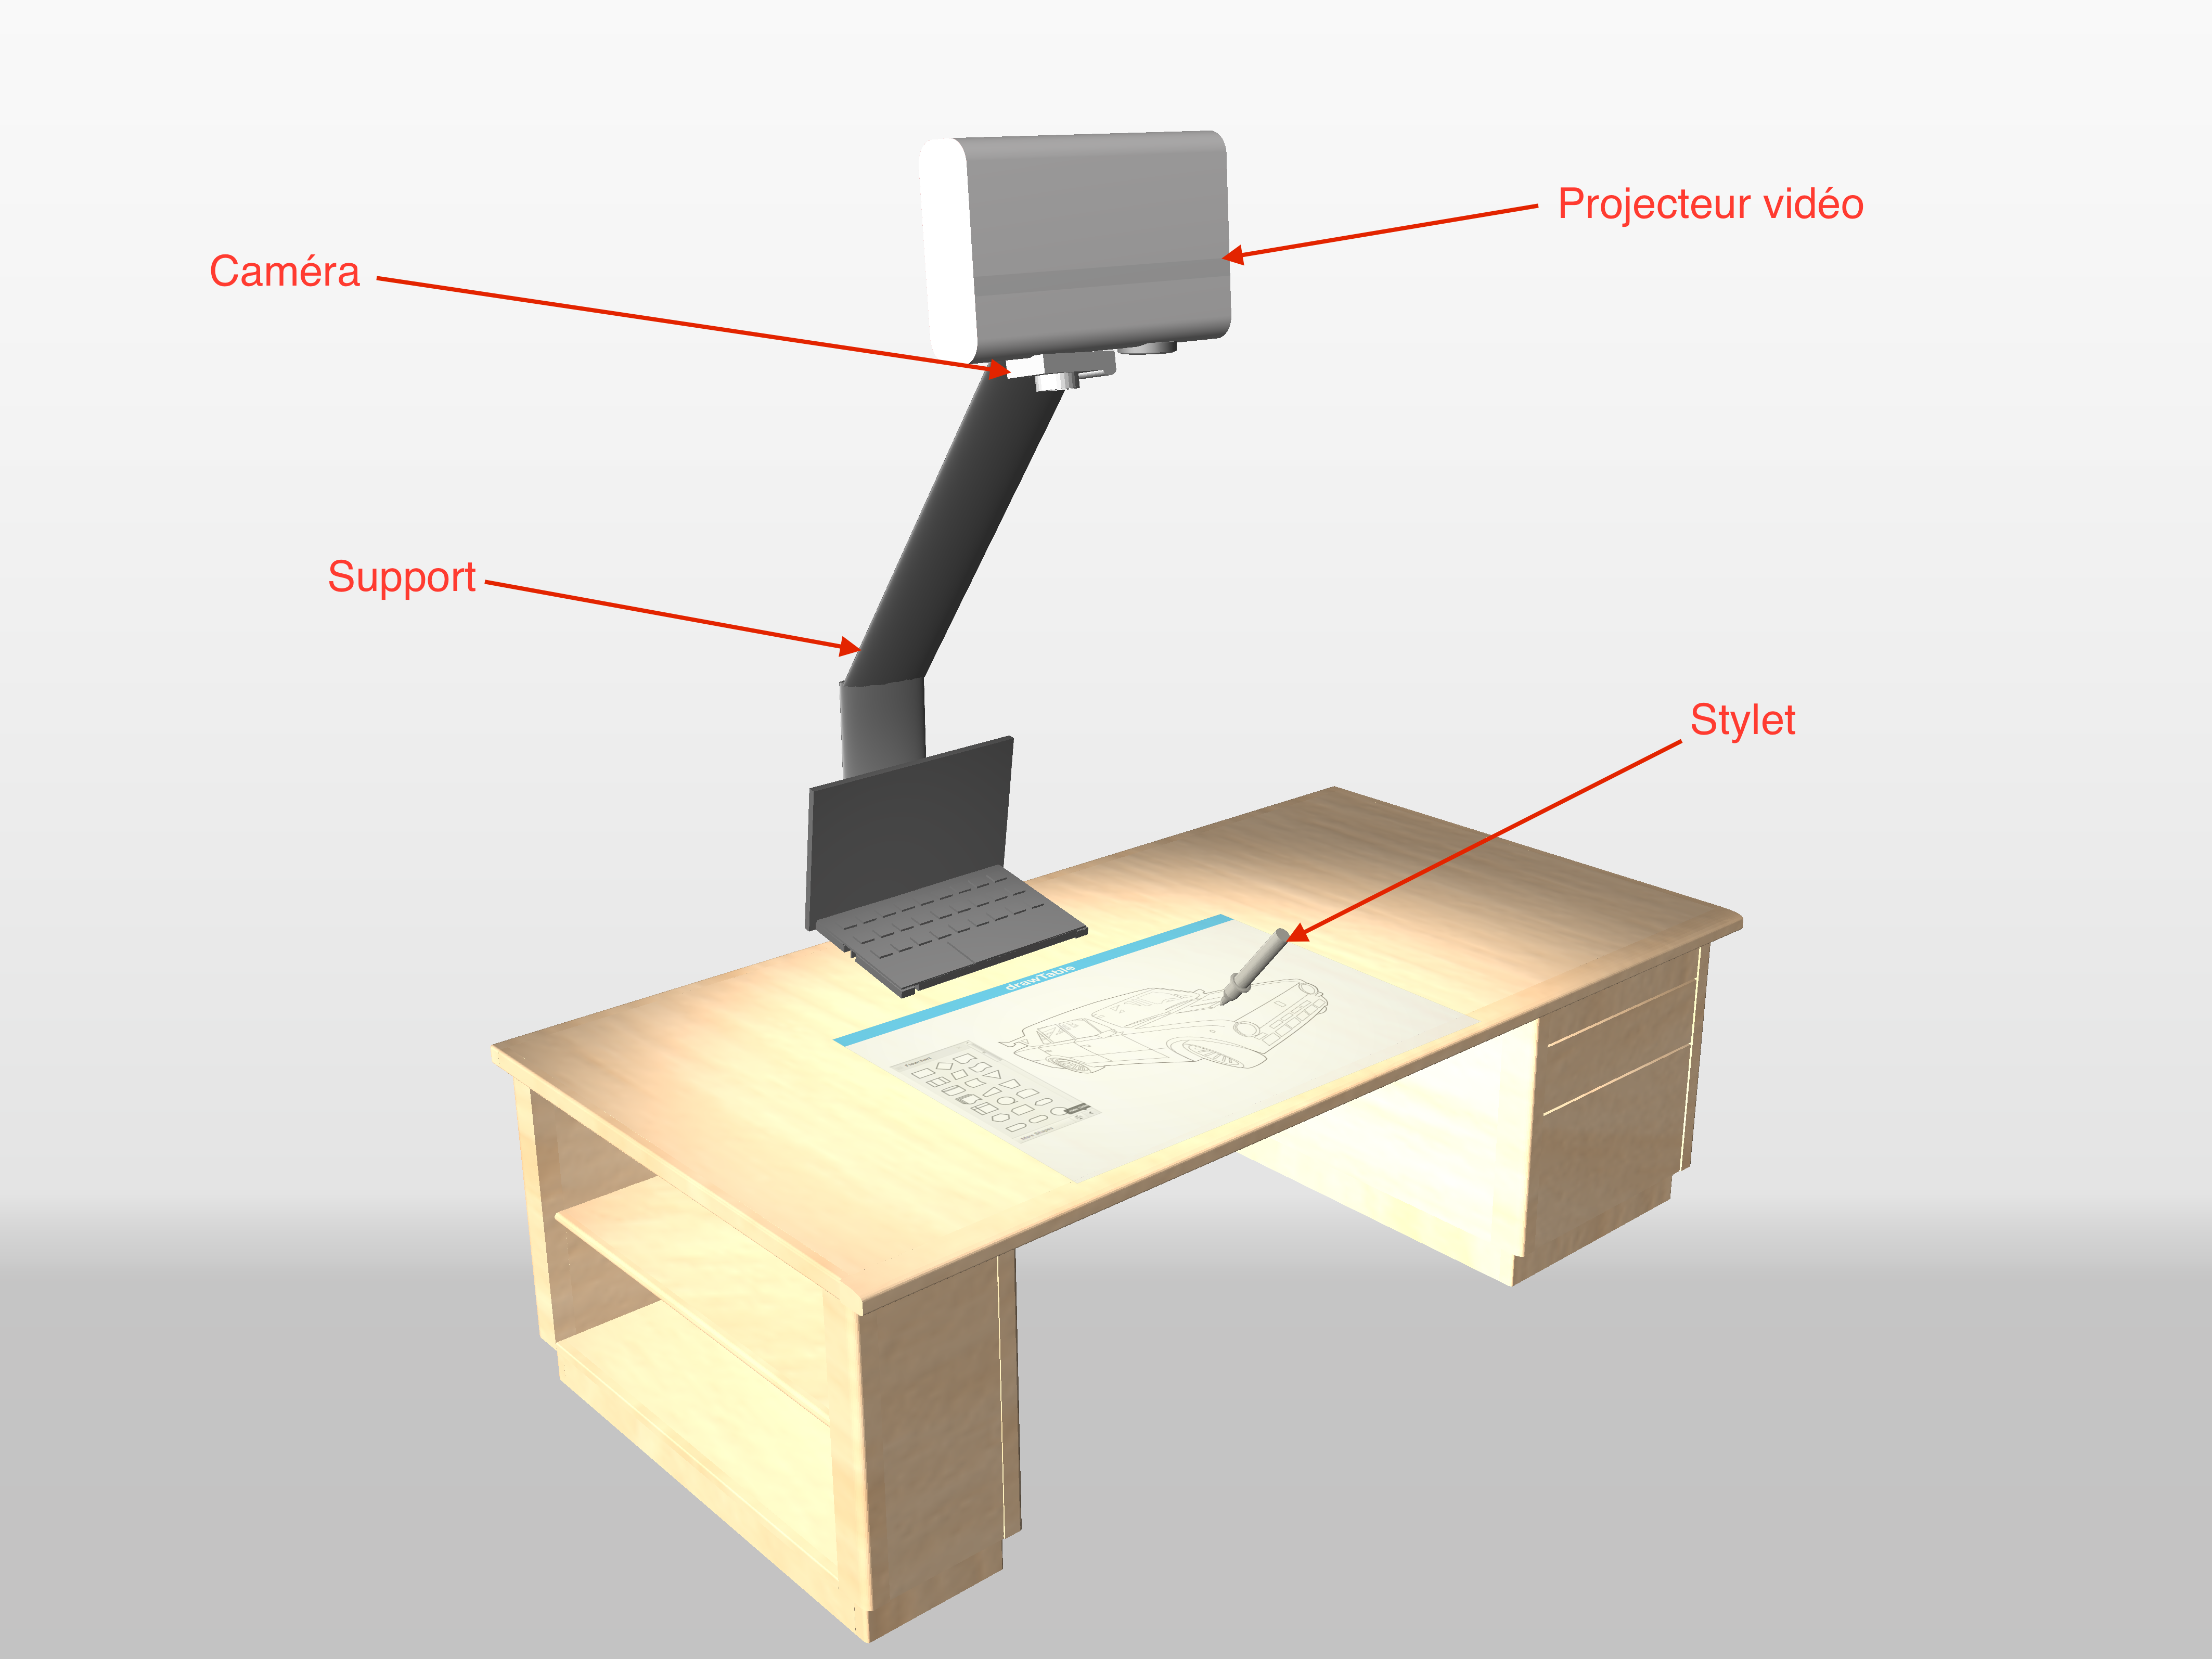
\includegraphics[angle=90, scale=0.15]{images/drawing-environment.png}
\caption{Exemple d'environnement de dessin - vue en perspective}
\end{figure}

\newpage

\begin{figure}[h]
\centering
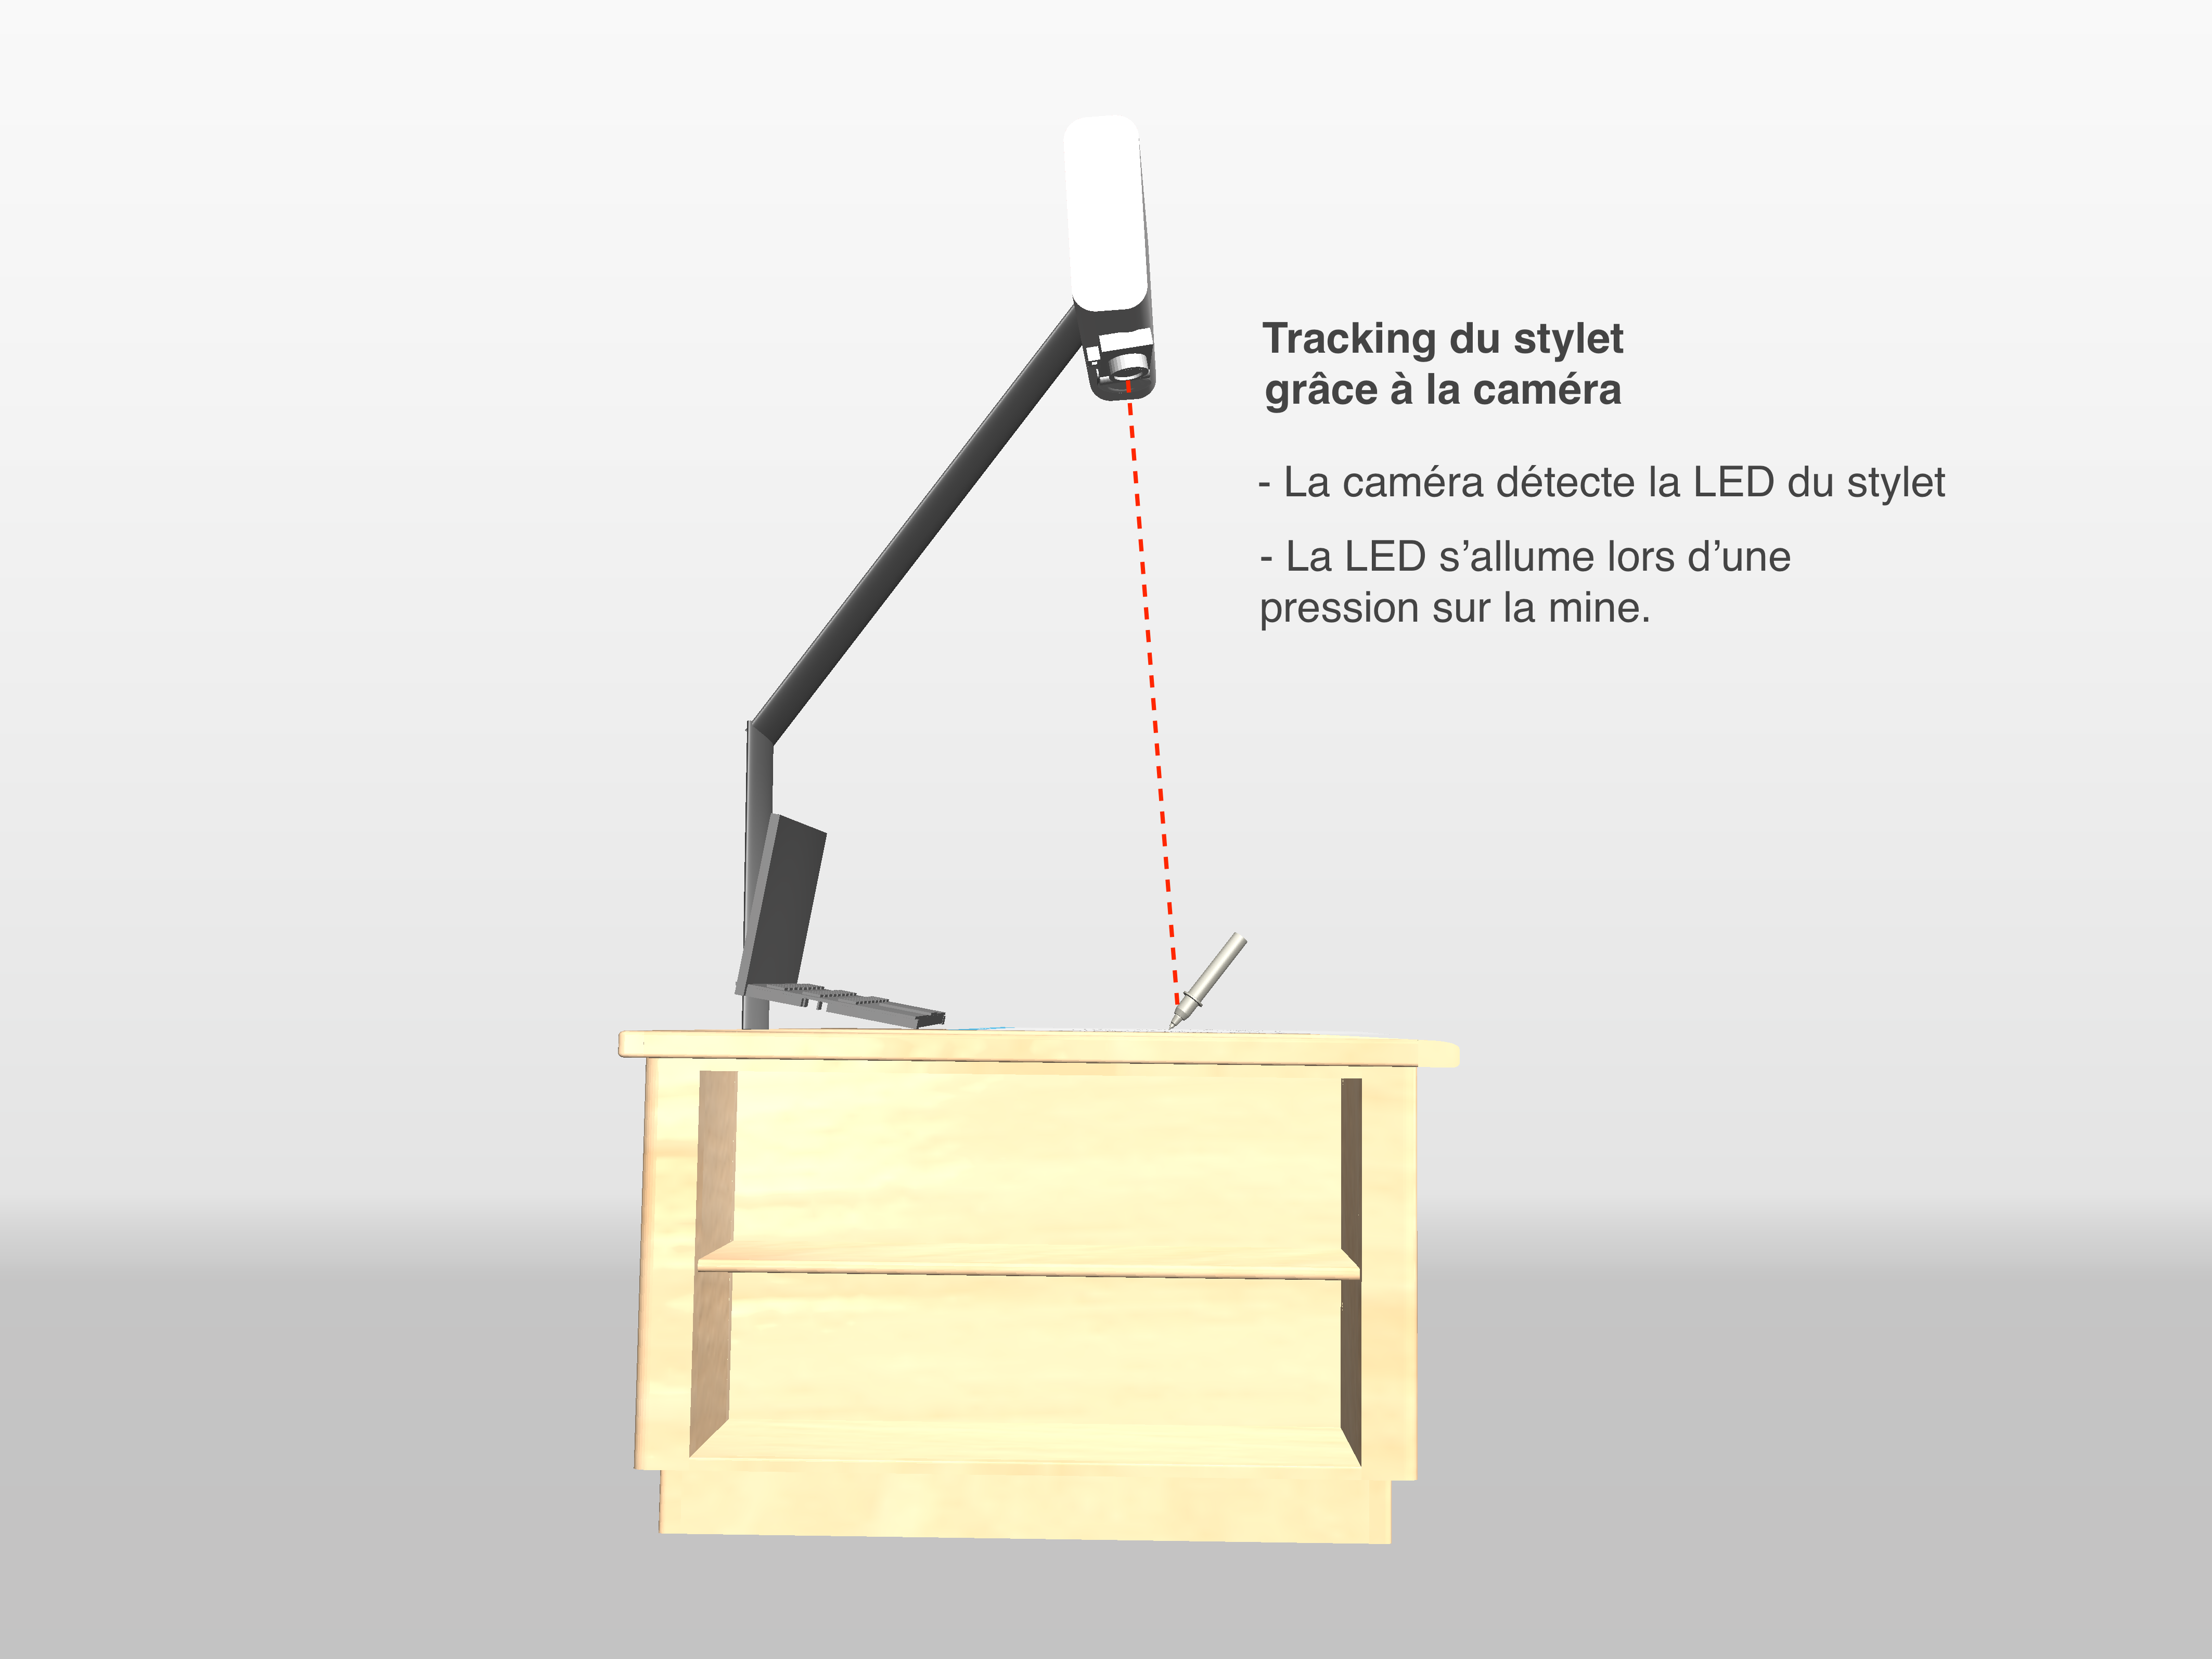
\includegraphics[angle=90, scale=0.15]{images/drawing-environment-side.png}
\caption{Exemple d'environnement de dessin - vue de gauche}
\end{figure}

%----------------------------------------------------------------------------------------
%	DESCRIPTION TECHNIQUE
%----------------------------------------------------------------------------------------

\chapter{Description technique}

\section{Structure du projet}

\section{Patrons de conception}

\section{Librairies}

Plus que des librairies, ce sont deux puissants frameworks qui ont été utilisé sur ce projet. 

\subsection{Qt}

Qt est un framework multi-plateforme en C++ permettant le développement de grosse application graphique. Son plus grand avantage est de fournir une couche d'abstraction aux API graphiques de Windows, Mac OS X, GTK, etc. Ainsi, la création et la gestion des éléments graphiques de l'application se fait de manière uniforme au travers des méthodes fournies par Qt.

Afin de proposer des mécanismes plus haut niveau que ceux inclus dans C++, Qt met à disposition un pré-compilateur (qmake) qui transformera certaine partie du code propre à Qt (les Q\_OBJECT, notamment) en C++. Il s'occupera aussi de la génération d'un Makefile compatible avec les différentes plateformes.

Dans ce projet, nous avons beaucoup utilisé Qt pour la gestion de fenêtre, mais aussi pour l'environnement de dessin. En effet, Qt met aussi à disposition des éléments comme la zone de dessin, la sélection et la gestion de couleur, etc.

\subsection{OpenCV}

OpenCV est un framework destiné au traitement en temps réel des images. Dans ce projet, nous l'avons surtout utilisé pour suivre le stylet de l'utilisateur et pouvoir ainsi reporter sa position dans le monde réel au référentiel de l'écran. Les algorithmes rapides d'OpenCV permettant de filtrer des couleurs, de travailler sur des formes géométriques et de faire des projections tridimensionnelles nous ont été très utiles.

\newpage

\section{Interface graphique utilisateur}

Cette section présente l'interface graphique utilisateur de l'application. Cette présentation débute par une introduction de sa structure. Elle est suivie d'une décomposition de ses différents constituants. Chaque constituant fait l'objet d'une description individuelle tant sur sa forme que sur son contenu.

L'interface graphique utilisateur a été développée de manière à ce que l'interaction du stylet avec celle-ci soit la plus agréable, la plus naturelle et la plus ergonomique que possible. Compte tenu du fait que le stylet peut s'avérer quelques peu moins précis que la souris de d'un ordinateur et ce, quel que soit la qualité du système de tracking, les éléments cliquables de l'interface utilisateur doivent en conséquent être adaptés. Concrètement, la taille des éléments doit être ajustée, c'est-à-dire être plus grands qu'ils ne le seraient dans le cas d'une application desktop traditionnelle.

Les applications susceptibles d'être développées pour des dispositifs tels que des smartphones et/ou des tablettes font l'objet d'une telle problématique. En effet, les éléments graphiques susceptibles de réagir à une action utilisateur sont plus grands qu'usuellement de manière à ce que l'interaction avec le doigt d'une personne soit aisée. Cette remarque s'applique également à cette application de dessin avec pour seule différence que les interactions s'effectuent par le biais d'un stylet.

Les éléments de l'interface graphique utilisateur ont été développés selon la problématique exposée dans le paragraphe précédent. En conséquence, l'interface dispose d'éléments graphiques plus grands. Par ailleurs, ces éléments sont la plupart du temps caractérisés par des icônes plutôt que par du texte devant décrire l'action qu'ils sont supposés représenter, une image étant souvent bien plus explicite que des mots si elle est bien choisie.

\subsection{Structure de l'interface utilisateur}

La figure suivante présente l'interface graphique utilisateur finale de l'application:

\begin{figure}[H]
\centering
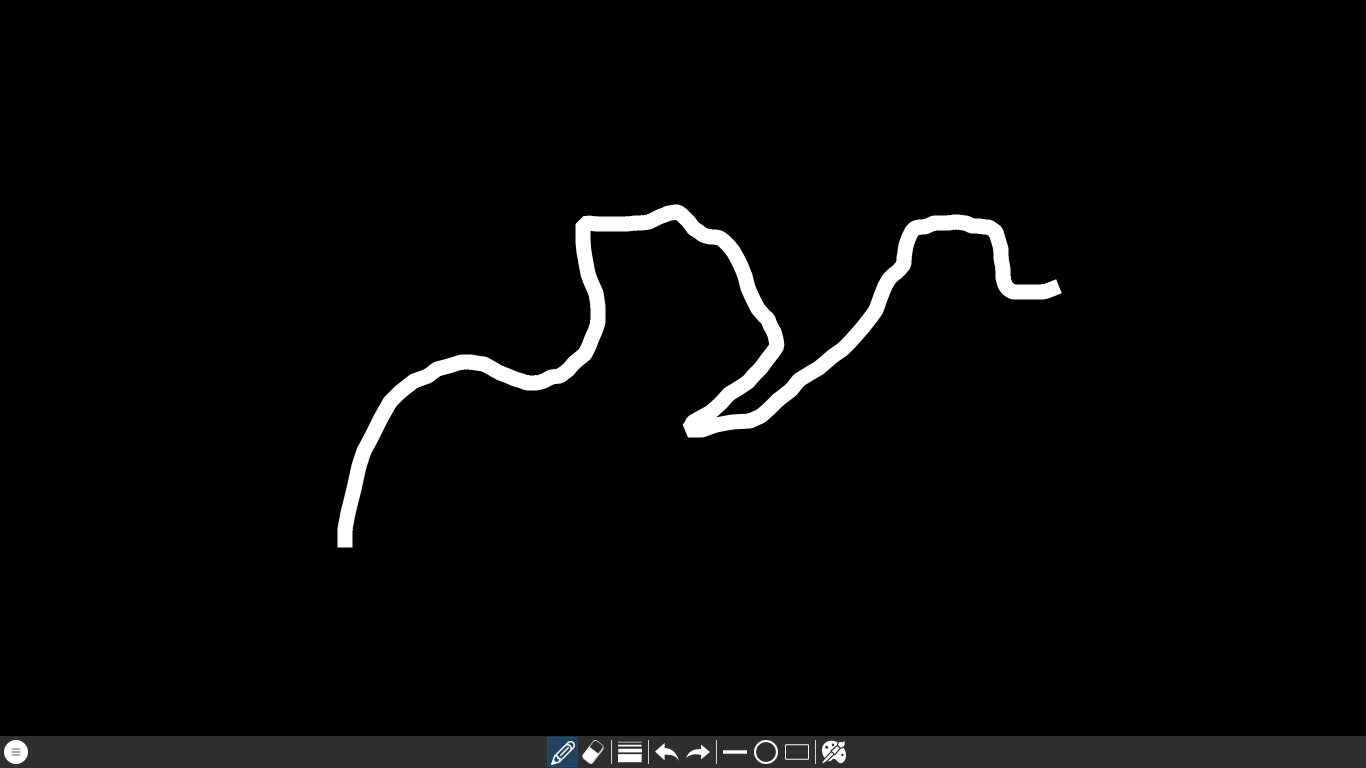
\includegraphics[scale=0.4]{images/ui-final.png}
\caption{Interface graphique utilisateur finale}
\end{figure}

La figure suivante présente la structure de l'interface graphique utilisateur finale de l'application:

\begin{figure}[h]
\centering
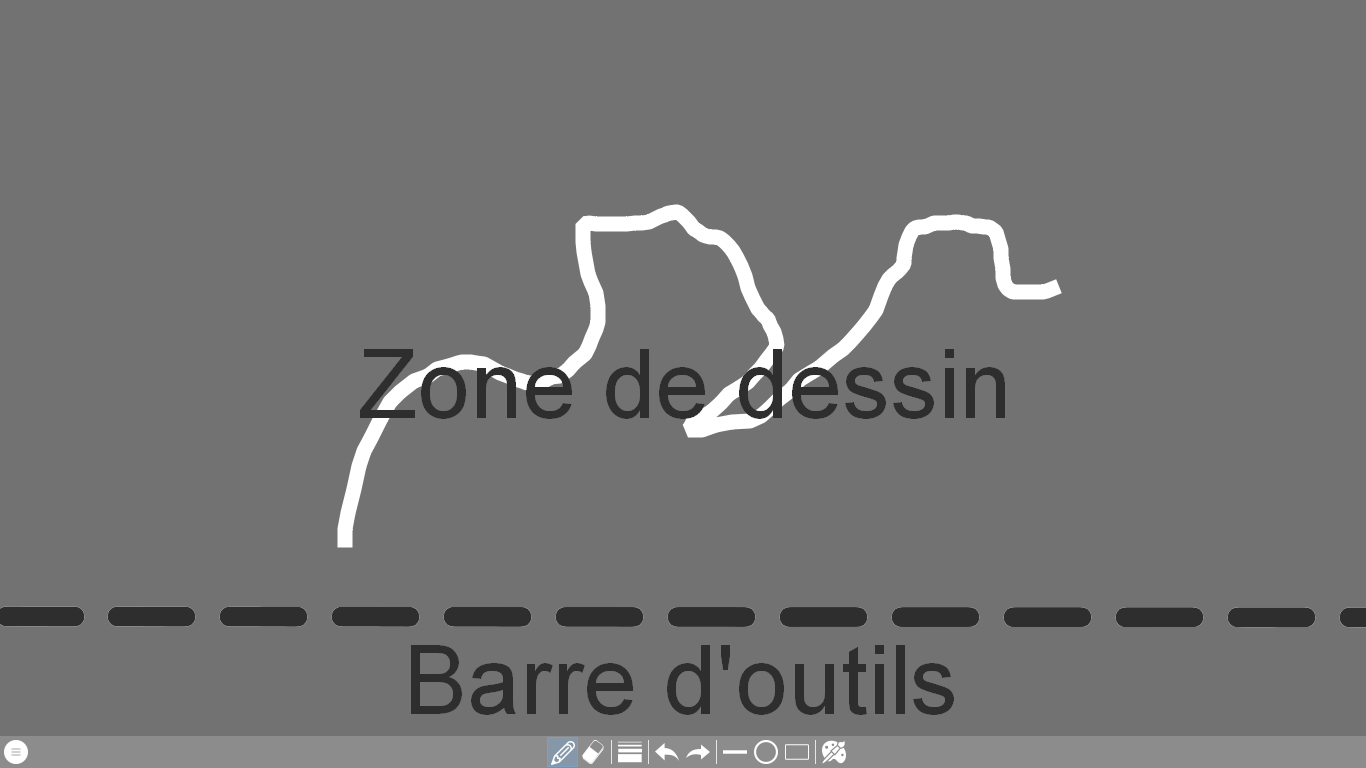
\includegraphics[scale=0.4]{images/ui-final-structure.png}
\caption{Structure de l'interface graphique utilisateur finale}
\end{figure}

La structure de l'interface graphique utilisateur est relativement rudimentaire; elle dispose d'une part d'une zone de dessin dans laquelle l'utilisateur est supposé y dessiner. D'autre part, elle dispose d'une barre d'outils laquelle fournit des outils de dessin, des outils de formes, des outils de couleurs et des outils d'épaisseur. Par ailleurs, cette barre d'outils met à disposition un outil supplémentaire permettant d'afficher le menu de l'application.

En termes d'implémentation, cette interface graphique utilisateur correspond à la classe MainWindow. Celle-ci hérite de la classe graphique QMainWindow. Cette classe fournie par le framework Qt propose entre autres une structure de base pour des applications caractérisées par une barre de menus, par une barre d'outils, par une zone centrale et par une éventuelle barre d'état. 

Dans le cas de l'application de dessin, la barre de menus n'est pas conservée dans la mesure où un menu personnalisé a été développé pour des raisons ergonomiques et est mis à disposition de l'utilisateur au moyen d'une boîte de dialogue. La zone centrale et la barre d'outils y figurent en ce qui les concernent. Pour ce qui est de la barre d'état, elle n'a pas été ajoutée à l'interface étant donné que son utilité pour une telle application ne présente que peu d'intérêt.

Il peut être constaté que l'interface utilisateur n'est pas caractérisée par une barre de titre que l'on rencontre dans les programmes fenêtrées. En effet, dès le lancement de l'application est affichée en mode plein écran. Il s'agit-là du mode par défaut de l'application qui ne peut faire l'objet d'une modification. Cela se justifie par le fait que le système de tracking analyse la totalité de l'écran et que l'affichage d'une partie d'une fenêtre native du système d'exploitation pourrait dégrader la qualité de détection du stylet d'une part, le mécanisme de calibrage d'autre part.

En dernière instance, l'ébauche de l'interface graphique définie lors de l'établissement du cahier des charges a été adaptée selon les besoins ergonomiques de l'application de dessin.

\subsection{Zone de dessin}

La figure suivante illustre la zone de dessin de l'application de dessin:

\begin{figure}[h]
\centering
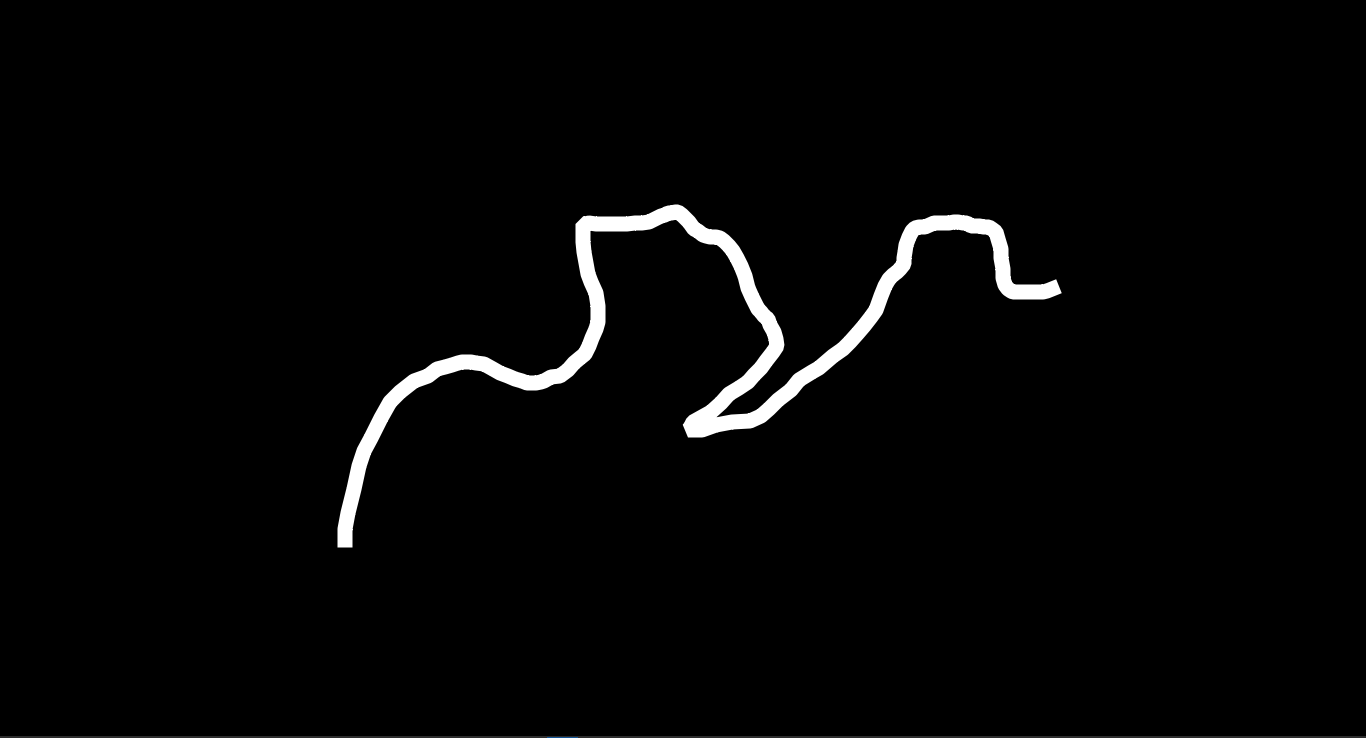
\includegraphics[scale=0.4]{images/drawing-area.png}
\caption{Zone de dessin}
\end{figure}

La zone de dessin consiste bien évidemment en un espace ouvert dans lequel il est possible à tout un chacun d'y esquisser son dessin. Aussi, si ce n'est cet espace, aucun autre élément graphique n'y figure à l'exception des éventuelles esquisses de l'utilisateur. Dans le cas de la figure précédente, il s'agit simplement d'une esquisse réalisée à l'aide de l'outil crayon.

En termes d'implémentation, cette zone de dessin correspond à la classe Drawing. Il s'agit de la vue du dessin, c'est-à-dire de la représentation virtuelle du dessin esquissé sur le support physique de l'utilisateur. Cette classe fait l'objet d'une spécialisation de la classe graphique QGraphicsView mise à disposition par le framework Qt.

\newpage

\subsection{Barre d'outils}

La figure suivante illustre la barre d'outils de l'application de dessin:

\begin{figure}[h]
\centering

\includegraphics[scale=0.4]{images/toolbar.png}
\caption{Barre d'outils}
\end{figure}

La barre d'outils propose les outils suivants selon leur ordre d'apparition:

\begin{table}[h]
\centering
\begin{tabular}{|l|l|l|}
\hline
\multicolumn{1}{|c|}{\textbf{Outil}} & \multicolumn{1}{c|}{\textbf{Icône}} & \multicolumn{1}{c|}{\textbf{Action}} \\ \hline
Menu                                 & 
\includegraphics{images/icon-menu.png}                                    & Déclenche l'ouverture du menu de l'application.                                                    \\ \hline
Crayon                               & 
\includegraphics{images/icon-pen.png}                                     & Déclenche la sélection de l'outil crayon.                                                         \\ \hline
Gomme                                & 
\includegraphics{images/icon-eraser.png}                                     & Déclenche la sélection de l'outil gomme.                                                          \\ \hline
Épaisseur                            & 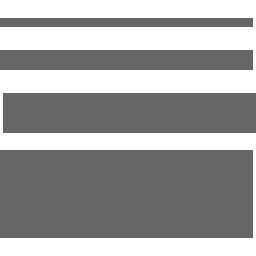
\includegraphics[scale=0.13]{images/icon-thickness.png}                                     & Déclenche l'ouverture d'un menu de sélection d'épaisseur.                                        \\ \hline
Annuler                              & 
\includegraphics{images/icon-undo.png}                                      & Annule la dernière action utilisateur sur le dessin.                                               \\ \hline
Rétablir                             & 
\includegraphics{images/icon-redo.png}                                     & Rétablit la dernière action utilisateur sur le dessin.                                             \\ \hline
Trait                                & 
\includegraphics{images/icon-dash.png}                                     & Déclenche la sélection de l'outil trait.                                                           \\ \hline
Cercle                               & 
\includegraphics{images/icon-ellipse.png}                                      & Déclenche la sélection de l'outil cercle.                                                          \\ \hline
Rectangle                            & 
\includegraphics{images/icon-rectangle.png}                                      & Déclenche la sélection de l'outil rectangle.                                                       \\ \hline
Couleur                              & 
\includegraphics{images/icon-color.png}                                      & Déclenche l'ouverture de la palette d'outils.                                                      \\ \hline
\end{tabular}
\caption{Outils de la barre d'outils de l'interface graphique utilisateur}
\end{table}

La sélection d'un outil peut avoir pour conséquence la modification de l'icône du curseur selon l'outil donné. Ceci améliore l'expérience utilisateur dans la mesure où le curseur représente au mieux l'outil actuellement manipulé. Ainsi, la sélection de l'outil crayon aura pour conséquence l'affiche d'un curseur avec une icône représentant un crayon. En termes d'implémentation, la barre d'outils correspond directement à un objet de la classe QToolBar fournie par le framework Qt. Il n'a pas été jugé nécessaire d'en faire une spécialisation compte tenu du fait qu'elle proposait déjà toutes les fonctionnalités nécessaires à l'application. Par ailleurs, cette barre d'outils fait l'objet d'une personnalisation visuelle plutôt que de laisser le style de barre natif du système hôte. Ceci est réalisé par le CSS suivant:

\begin{lstlisting}[
           caption=CSS de la barre d'outils de l'interface graphique utilisateur,
           showspaces=false,
           basicstyle=\ttfamily,
           numbers=left,
           numberstyle=\tiny,
           commentstyle=\color{gray}
        ]
QToolBar{ 
    background: rgb(46,46,46); 
    border: 0px; 
}
\end{lstlisting}

\newpage

\subsection{Menu}

\subsection{Ressources}

\section{Tracking}

\subsection{Système de détection}

\subsection{Mouvement du stylet}

\subsection{Déclenchement du dessin}

\subsection{Filtrage de couleurs}

\subsection{Précision du tracking}

\subsection{Contraintes de luminosité}

\newpage

\section{Dessin}

\subsection{Outils de dessin}

\subsubsection{Crayon}

\subsubsection{Gomme}

\subsection{Outils de formes}

\subsubsection{Trait}

\subsubsection{Rectangle}

\subsubsection{Cercle}

\subsection{Outils de couleurs}

\subsubsection{Palette de couleurs}

\subsection{Choix d'épaisseur}

\section{Interfaçage tracking-dessin}

\subsection{Communication inter-projet}

\subsubsection{Modèle des sockets}

\subsubsection{Protocole de communication}

\subsubsection{Structure des messages}

\subsection{Simulation et contrôle de la souris}

\section{Historique des actions}

\section{Clavier virtuel}

\section{Sérialisation}

\subsection{Importation}

\subsection{Sauvegarde}

\subsection{Interface d'utilisation}

\section{Impression}

%----------------------------------------------------------------------------------------
%	PROCEDURE DE TESTS
%----------------------------------------------------------------------------------------

\chapter{Tests \& Validation}

\section{Stratégie de tests}

\section{Outils}

\section{Matériel}

\section{Procédures de tests}

\section{Résultats}

%----------------------------------------------------------------------------------------
%	PROBLEMES CONNUS
%----------------------------------------------------------------------------------------

\chapter{Problèmes connus}

%----------------------------------------------------------------------------------------
%	CONCLUSION
%----------------------------------------------------------------------------------------

\chapter{Conclusion}

\section{Solution proposée}

\subsection{Fonctionnalités implémentées}

\subsection{Fonctionnalités non implémentées}

\subsection{Propositions d'amélioration}

\textit{TODO: Infrarouge, avec caméra infrarouge (Wiimote)}

\textit{TODO: Amélioration du logiciel de dessin}

\section{Problèmes rencontrés}

\subsection{Problèmes organisationnels}

\subsection{Problèmes techniques}

\subsection{Problèmes de planification}

\section{Respect du planning}

\subsection{Planification initiale}

\subsection{Évolution}

\textit{TODO: pas facile d'imaginer un planning sur quelque chose que l'on a jamais fait, sur quelque chose d'expérimental, finalement, le tracking aura duré durant tout le projet, on peut tout le temps l'améliorer}

\section{Déroulement du projet}

\subsection{Points positifs}

\textit{TODO: On a appris plein de truc: OpenCV, tracking, caméra, la difficulté de gérer un projet difficile à tester}

\subsection{Points négatifs}

\section{Synthèse}

%----------------------------------------------------------------------------------------
%	LISTINGS
%----------------------------------------------------------------------------------------

\lstlistoflistings

%----------------------------------------------------------------------------------------
%	APPENDIX
%----------------------------------------------------------------------------------------

\appendix

%----------------------------------------------------------------------------------------
%	CAHIER DES CHARGES
%------------------------------------------------------------------------------s----------

\chapter{Cahier des charges}

\section{Contexte}

Ce projet de groupe se déroule dans le cadre de la formation Bachelor HES de la Haute-Ecole d'Ingénierie et de Gestion du canton de Vaud. Il compte pour une unité d'enseignement du plan d'étude de l'orientation Informatique logiciel (IL) du département des Technologies de l'Information et de la Communication (TIC) de l'école. Il se réalise durant le cinquième semestre de l'année de formation 2015/16.

\section{Membres du groupe}

Les personnes suivantes constituent les membres du groupe de l'équipe de projet:

\begin{itemize}
\item[$\bullet$] Sacha Bron - \textit{Chef de groupe}
\item[$\bullet$] David Villa - \textit{Chef suppléant}
\item[$\bullet$] Paul Ntawuruhunga
\item[$\bullet$] Yassin Kammoun
\item[$\bullet$] Marc Pellet
\end{itemize}

\section{Objectif du projet}

L'objectif de ce projet est de concevoir un outil de dessin assisté par ordinateur permettant à l'utilisateur de réaliser ses dessins de la manière la plus naturelle possible. À terme, l'utilisateur dessinera directement sur sa table ou n'importe quelle autre surface plane à l'aide d'un stylet et son dessin sera projeté sur son plan de travail, donnant à l'utilisateur l'impression de dessiner avec un crayon et une feuille.

\section{Fonctionnalités principales}

Les fonctionnalités principales du projet sont les suivantes:

\begin{itemize}
\item[$\bullet$] Dessin à l’aide d’un stylet.
\item[$\bullet$] Projection de l’image sur le plan de travail.
\item[$\bullet$] Alignement de l’image avec la position du stylet.
\item[$\bullet$] Calibrage du stylet.
\item[$\bullet$] Plan de travail avec barre d'outils.
    \begin{itemize}
	\item Une barre d'outils sera projetée dans une zone du plan travail permettant à l'utilisateur de sélectionner un outil.
	\begin{itemize}
    \item[$\circ$] Outils de dessin: crayon, gomme.
	\item[$\circ$] Outils de forme: ligne droite, carré, cercle.
	\item[$\circ$] Outils de couleur: palette de couleurs.
	\item[$\circ$] Outils de choix d'épaisseur.
	\end{itemize}
    \end{itemize}
\item[$\bullet$] Annulation d’une action
    \begin{itemize}
	\item Une pile d'actions est enregistrée et un bouton dans la barre d'outils permet de remonter cette pile, annulant ainsi les dernières modifications apportées au dessin.
	\end{itemize}
\item[$\bullet$] Enregistrement et importation du dessin
	\begin{itemize}
	\item Possibilité d'enregistrer ou importer son dessin au format PNG.
	\end{itemize}
\end{itemize}

\section{Fonctionnalités supplémentaires}

Les fonctionnalités supplémentaires du projet sont les suivantes:

\begin{itemize}
\item[$\bullet$] Site vitrine.
\item[$\bullet$] Pipette.
\item[$\bullet$] Remplissage.
\item[$\bullet$] Rétablissement d'une action.
\end{itemize}

\section{Mockup}

La figure suivante illustre une ébauche de l'interface graphique utilisateur devant correspondre au plan de travail:

\begin{figure}[h]
\centering
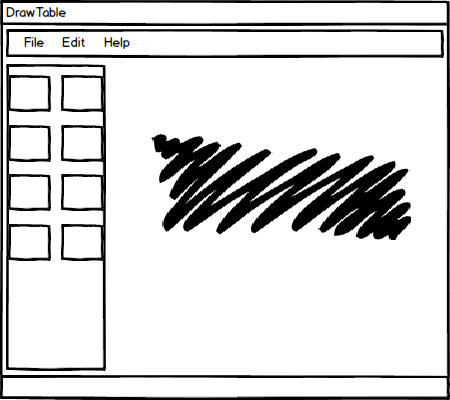
\includegraphics[scale=0.5]{images/ui.png}
\caption{Mockup de l'interface graphique utilisateur}
\end{figure}

L'interface graphique utilisateur est divisée en trois parties à savoir la barre des menus, la barre d'outils et la zone de dessin.

\section{Prototype du stylet}

Le prototype de stylet est conçu par le chef de projet. Sa conception nécessite les composants suivants:

\begin{itemize}
\item[$\bullet$] LED.
\item[$\bullet$] Un interrupteur.
\item[$\bullet$] Une résistance.
\item[$\bullet$] Une batterie.
\item[$\bullet$] Un boîtier.
\end{itemize}

La figure suivante propose une ébauche de prototype du stylet:

\newpage

\begin{figure}[h]
\centering
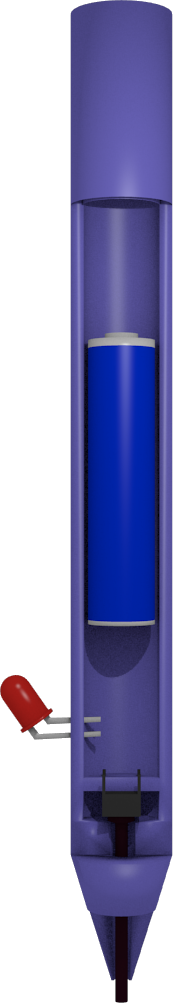
\includegraphics[scale=0.5]{images/stylus-first-design.png}
\caption{Prototype initial du stylet}
\end{figure}

\newpage

\section{Principe de fonctionnement}

Ce projet contient trois principales difficultés: la détection de contact du stylet sur la table, le suivi de la position du stylet (\textit{tracking}) et la précision de l'entier du système.

Pour cela nous avons imaginé un stylet muni d'une mine spéciale. Lors d'une pression sur le plan de travail, cette dernière presse sur un bouton qui enclenche une diode électroluminescente placée proche de la mine. Une caméra placée au-dessus du plan de travail filme la scène et envoie l'image au logiciel chargé de suivre la position de la mine du stylet en détectant cette LED.

Le programme de dessin récupère les coordonnées du stylet et les interprète de manière à pouvoir projeter le dessin sur le plan de travail à l'aide du projecteur vidéo.

L'application comportera différents threads: un thread de l'application sera consacré au tracking de la LED, un autre récupérera les coordonnées pour les interpréter sur le plan de travail en fonction de l'outil sélectionné.

\section{Public-cible}

L'application vise avant toute chose tout amateur de dessin souhaitant se passer d'une feuille. 

\section{Technologies utilisées}

Les technologies utilisées pour le développement de l'application et le suivi du stylet sont les suivantes:

\begin{itemize}
\item[$\bullet$] Librairie OpenCV - Pour le suivi du stylet en temps réel.
\item[$\bullet$] Framework Qt - Pour l'interface graphique du plan de travail.
\end{itemize}

\section{Matériel requis}

Les points suivants constituent le matériel requis pour l'utilisation de l'application.

\begin{itemize}
\item[$\bullet$] Un prototype de stylet faisant office d'outil de dessin.
\item[$\bullet$] Une caméra permettant de traquer les mouvements du stylet. 
\item[$\bullet$] Un projecteur vidéo permettant de retranscrire le dessin de l'utilisateur.
\item[$\bullet$] Un plan de travail permettant de dessiner.
\item[$\bullet$] Un support prévu pour la disposition de la caméra et du projecteur au-dessus du plan de travail.
\end{itemize}

\section{Plateformes supportées}

De par la nature du framework Qt, l'application est automatiquement multi-plateforme; elle est donc supportée par les environnements usuels. Il s'agit entre autres des éditions Windows, des systèmes Mac OS X et des différentes distributions Linux. Un simple travail de recompilation du code source sur l'environnement désiré permet de disposer d'une version compatible de l'application.

\section{Déploiement}

\subsection{Installation de l'application}

Le déploiement de l'application suit la procédure standard des environnements supportés:

\begin{itemize}
\item[$\bullet$] Pour un environnement Windows, le déploiement se réalise par le biais d'un installateur. 
\item[$\bullet$] Pour un environnement Mac OS X, le déploiement se réalise par le biais d'un fichier DMG.
\item[$\bullet$] Pour une distribution Linux (Arch), le déploiement se réalise par le biais d'un paquetage.
\end{itemize}

\subsection{Mise en place du matériel}

La mise en place du matériel requis est décrite par la procédure suivante:

\begin{enumerate}
\item  Disposez le support de travail.
\item  Posez le stylet sur le support de travail.
\item  Placez la caméra au-dessus du support de travail.
\item  Placez le projecteur vidéo au-dessus du support de travail.
\end{enumerate}

Les schémas suivants illustrent un environnement de travail idéal:

\newpage

\begin{figure}[H]
\centering
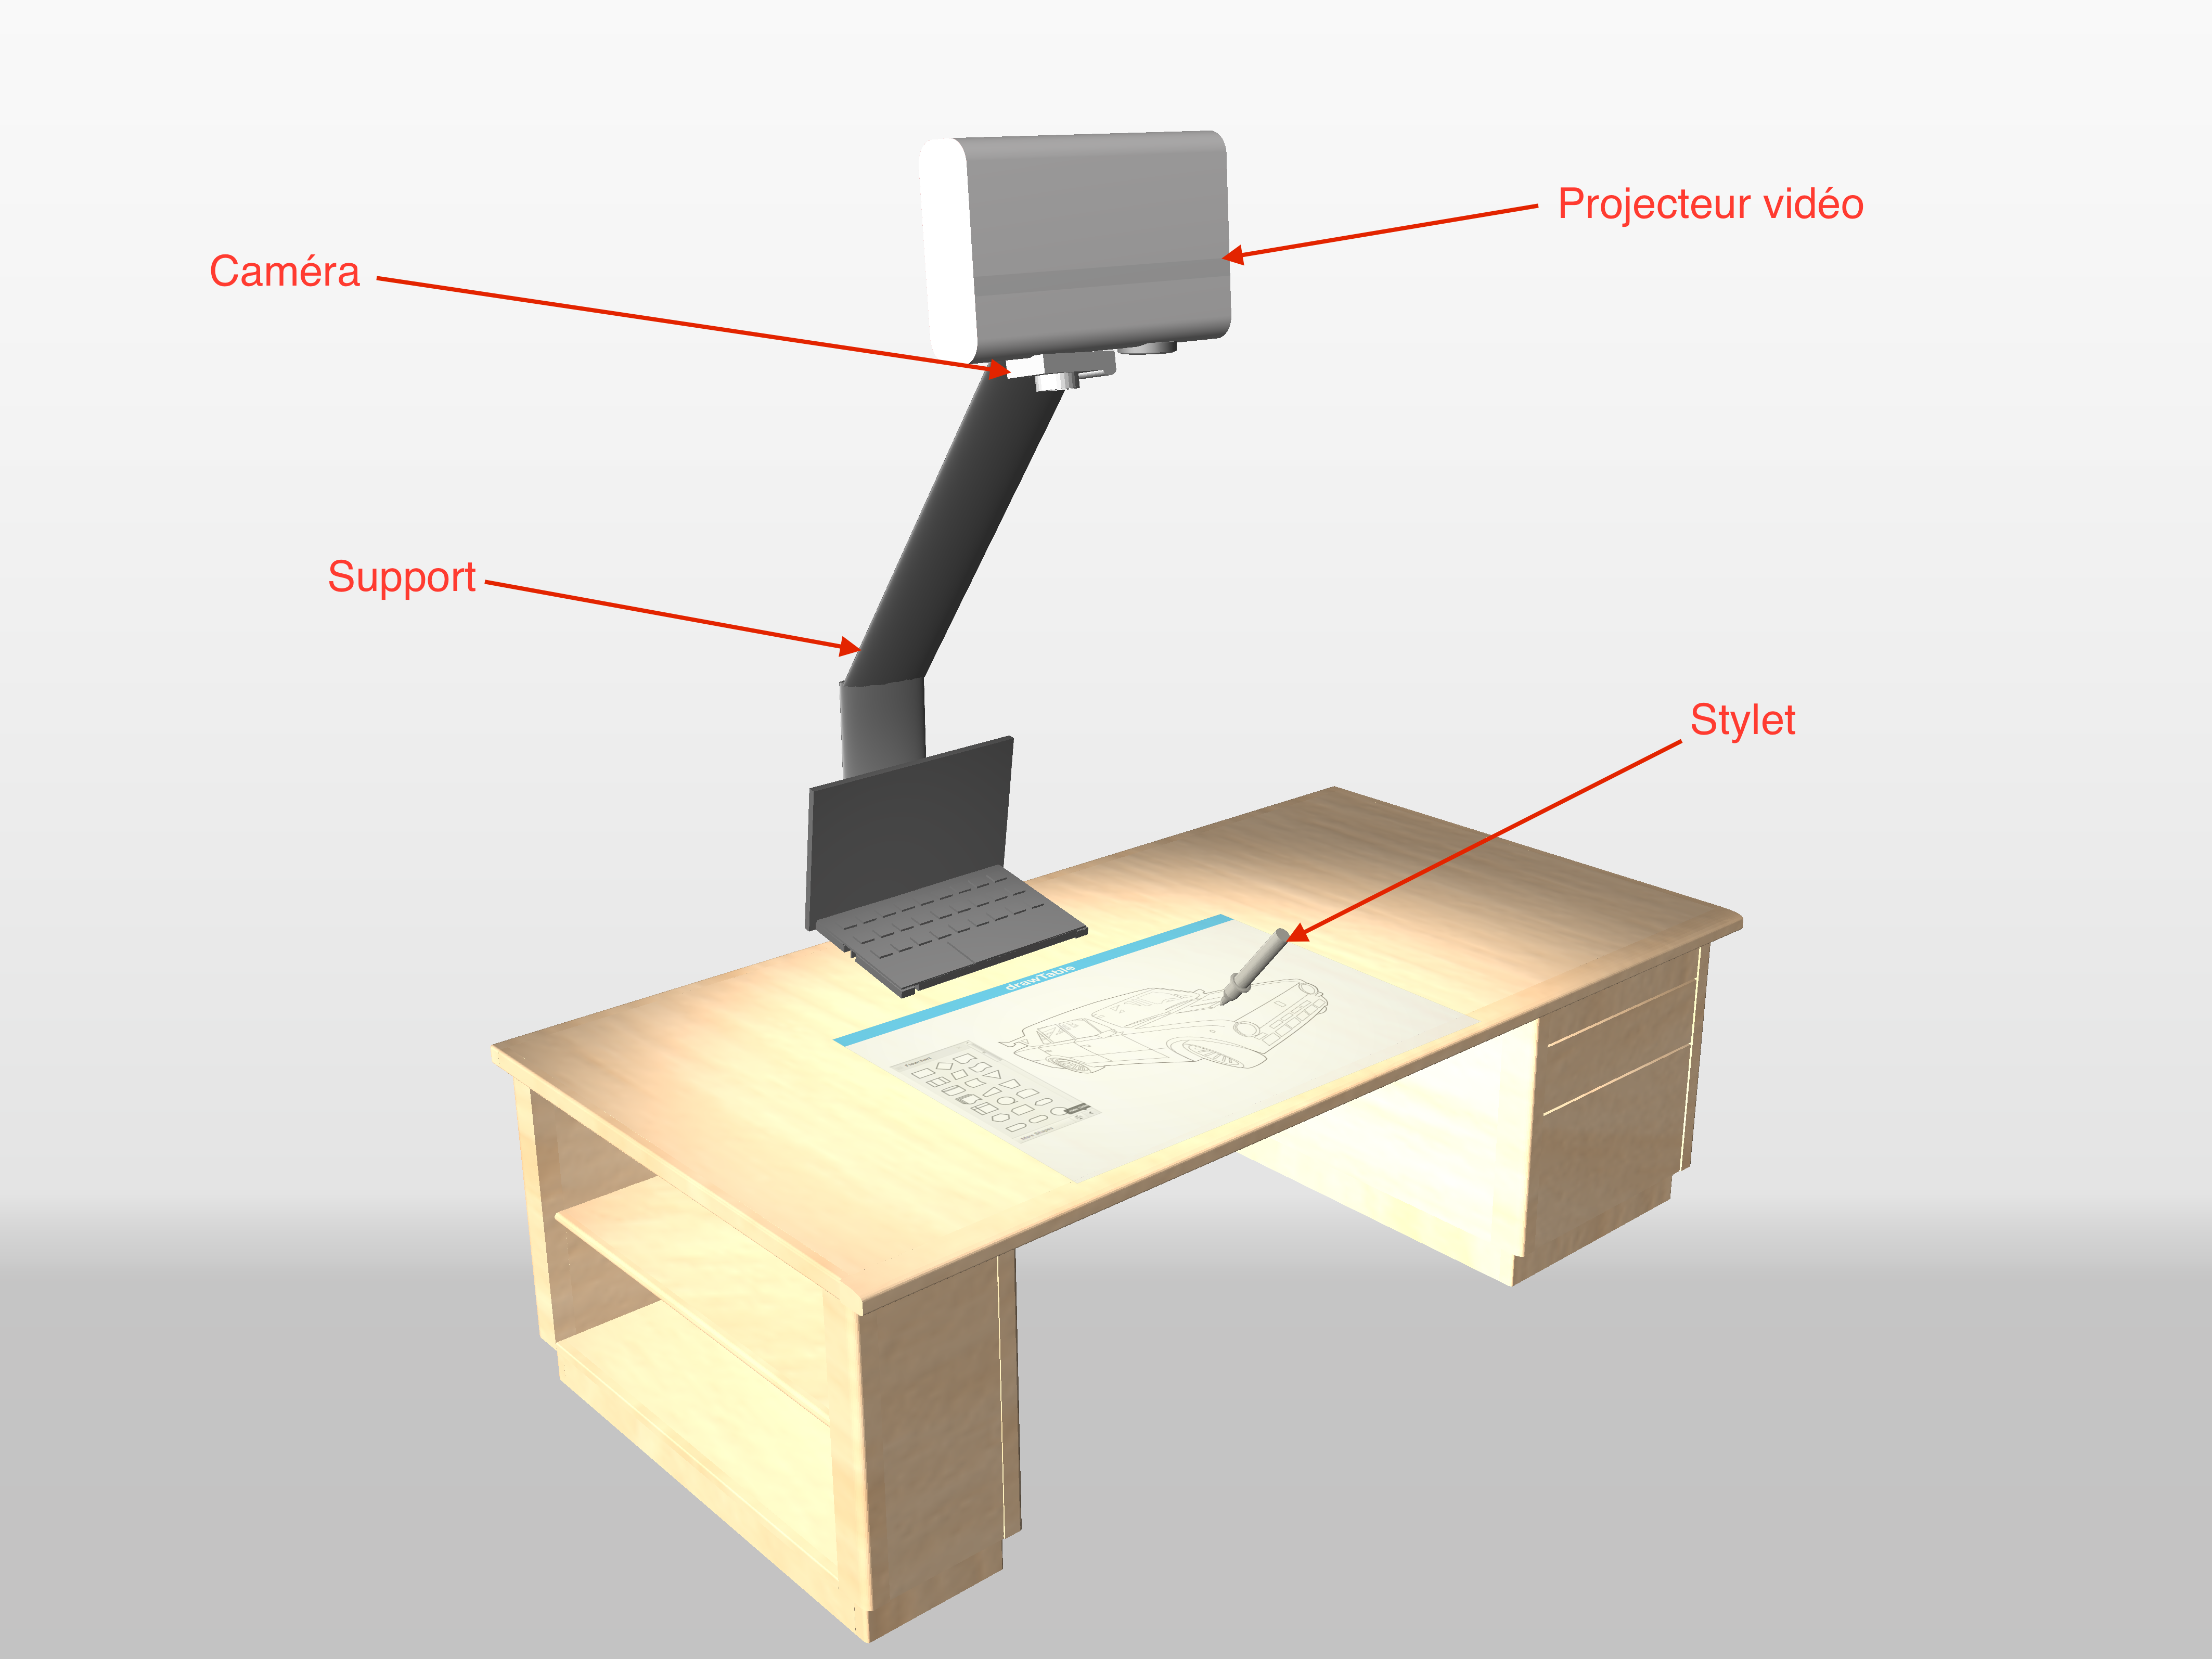
\includegraphics[angle=90, scale=0.15]{images/drawing-environment.png}
\caption{Vue en perspective d'un environnement idéal}
\end{figure}

\newpage

\begin{figure}[H]
\centering
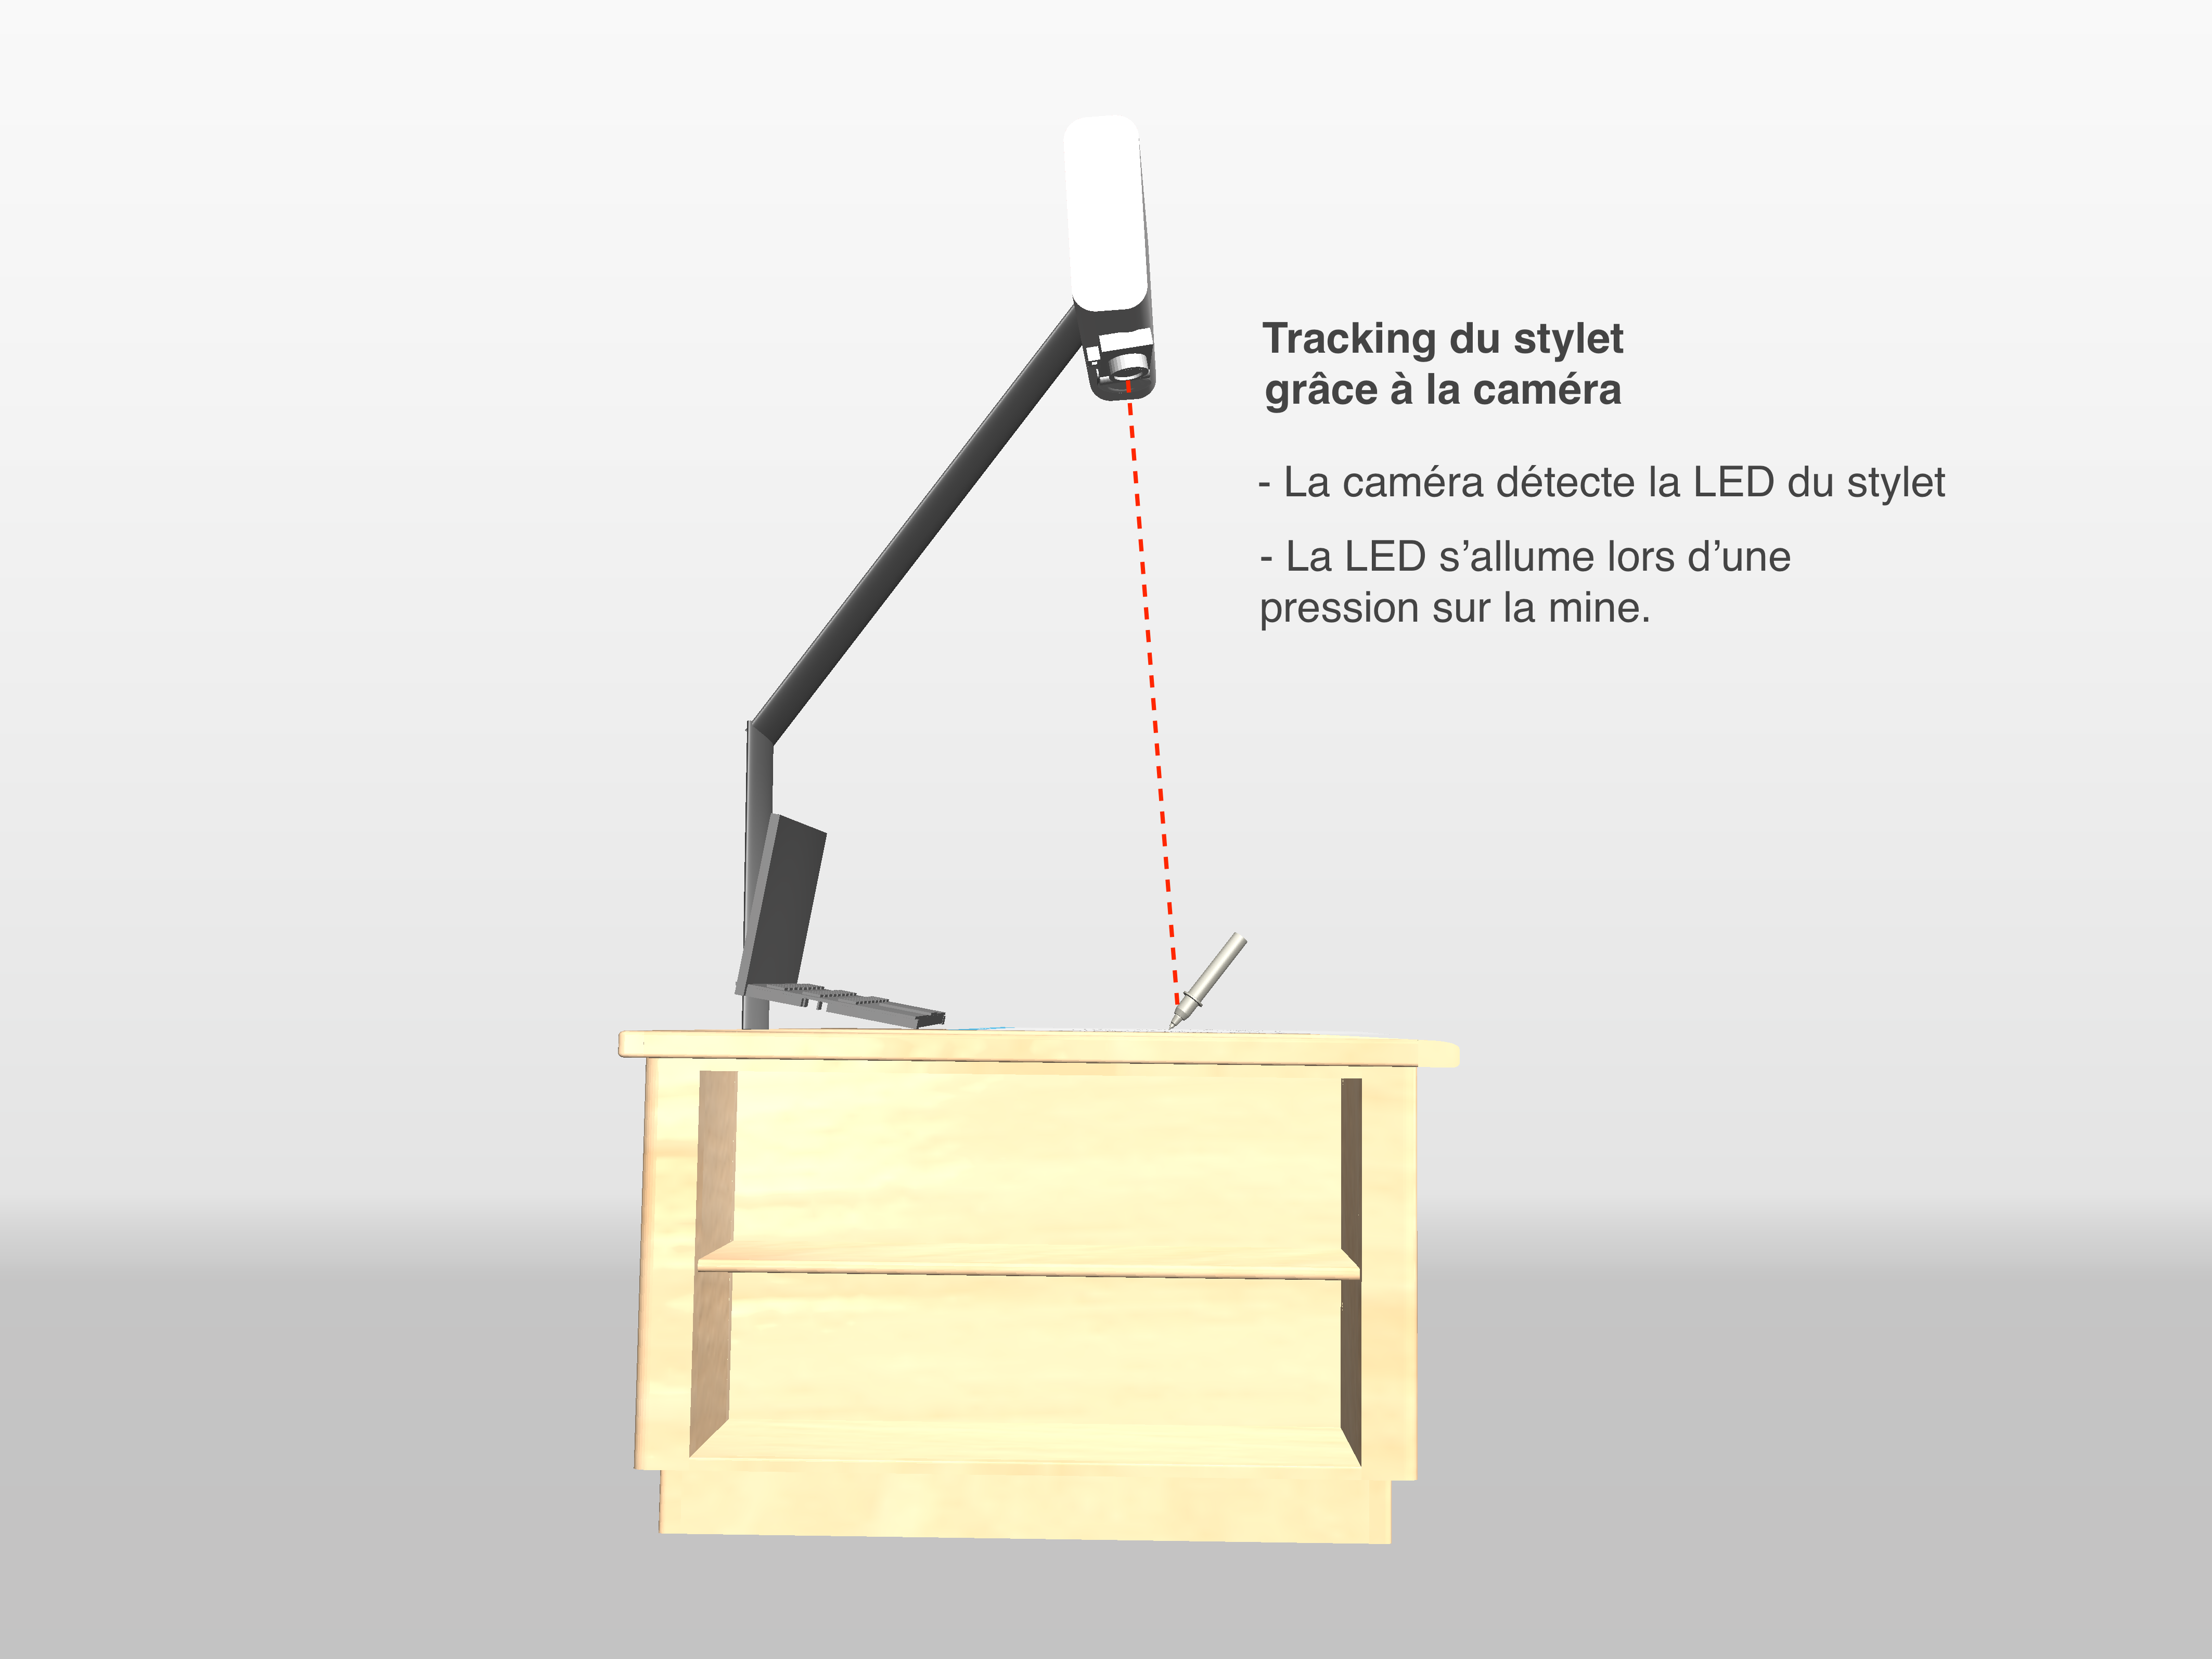
\includegraphics[angle=90, scale=0.15]{images/drawing-environment-side.png}
\caption{Vue de côté d'un environnement idéal}
\end{figure}

\newpage

\section{Déroulement du projet}

\subsection{Planification des tâches}

Le diagramme de Gantt qui suit présente la planification des tâches du projet:

\begin{figure}[H]
\centering
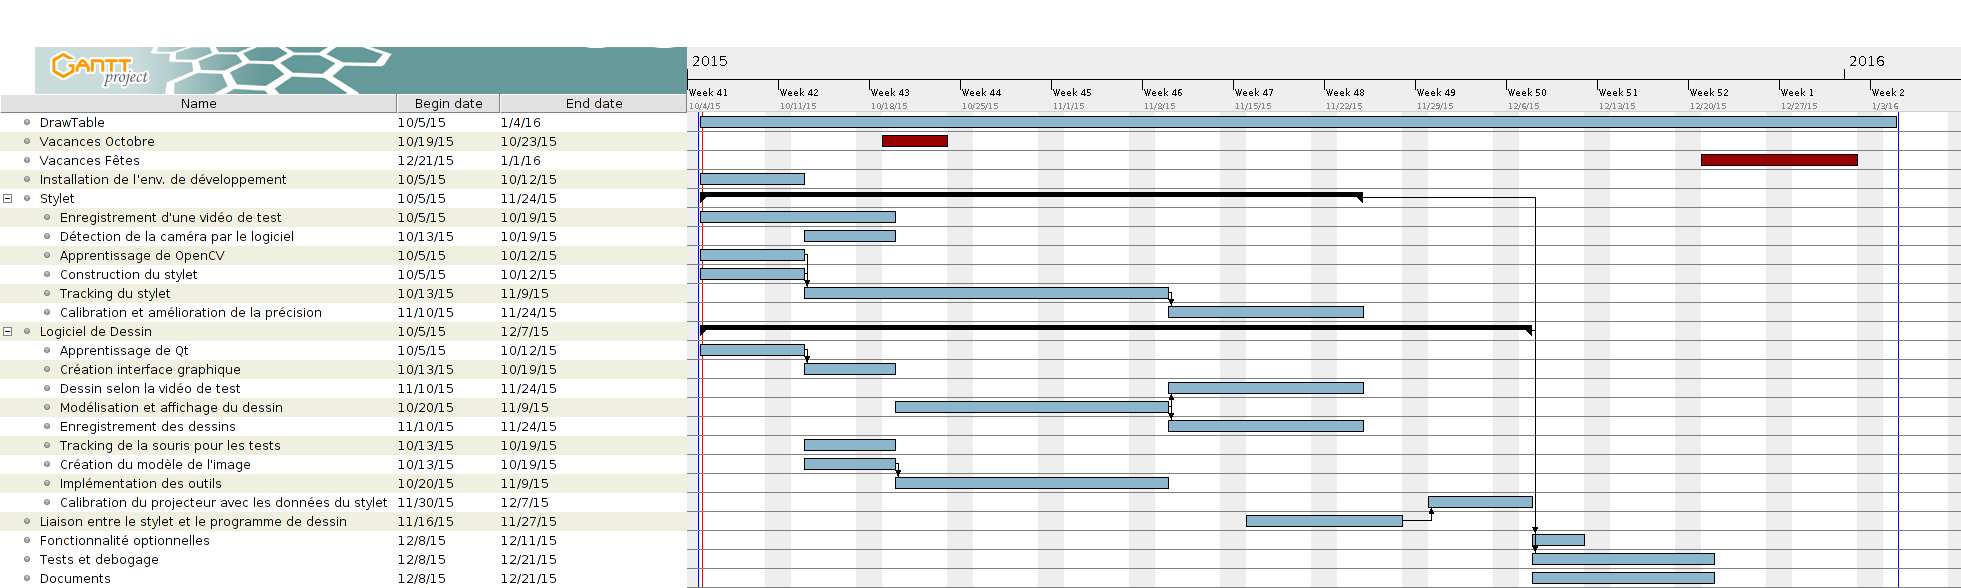
\includegraphics[angle=90, scale=0.3]{images/planification.png}
\caption{Planification initiale des tâches}
\end{figure}

\newpage

\subsection{Description des tâches}

Les points suivants constituent un bref descriptif des tâches du projet:

\begin{itemize}
\item[$\bullet$] Enregistrement d'une vidéo de test
    \begin{itemize}
	\item Afin de pouvoir tester les différents outils du logiciel de dessin avant que l'outil de tracking ne soit terminé, une vidéo contenant différents mouvements sera enregistrée.
	\end{itemize}
\item[$\bullet$] Apprentissage d'OpenCV
    \begin{itemize}
	\item Pour toutes les opérations de tracking du stylet, nous allons utiliser la librairie OpenCV. Il sera donc nécessaire de prendre le temps d’en apprendre les bases avant de se lancer à corps perdu dans l’implémentation.
	\end{itemize}
\item[$\bullet$] Construction d'un stylet
    \begin{itemize}
	\item Un stylet de notre propre création sera utilisé pour cette application, le matériel nécessaire à la fabrication de ce dernier est détaillé dans la description du prototype du stylet.
	\end{itemize}
\item[$\bullet$] Tracking du stylet
    \begin{itemize}
	\item A l’aide d’une caméra, nous détecterons les mouvements du stylet, il faudra donc récupérer ces informations et les transmettre au logiciel de dessin.
	\end{itemize}
\item[$\bullet$] Apprentissage de Qt
    \begin{itemize}
	\item Apprentissage des librairies Qt pour ce qui concerne principalement les interfaces graphiques et les librairies de dessin.
	\end{itemize}
\item[$\bullet$] Création de l’interface graphique
    \begin{itemize}
	\item Conception de l’interface graphique du logiciel. Celle-ci contiendra un menu permettant d’importer/exporter des images, d’un plan de travail sur lequel travailler ainsi qu’une boîte à outils contenant différentes fonctionnalités telles que le crayon, la gomme, une palette de couleurs, le choix de l’épaisseur du trait.
	\end{itemize}
\item[$\bullet$] Tracking intermédiaire de la souris
    \begin{itemize}
	\item Afin de permettre de tester le bon fonctionnement de l’implémentation des différents outils, ceci d’une manière accessible à tous les développeurs, il faut implémenter une fonctionnalité permettant de dessiner à l’aide de la souris.
	\end{itemize}
\item[$\bullet$] Création du modèle de l’image
    \begin{itemize}
	\item Conception et création du modèle qui sera utilisé par le logiciel pour représenter notre image.
	\end{itemize}
\item[$\bullet$] Implémentation des outils
    \begin{itemize}
	\item Implémentation des fonctionnalités obligatoires disponibles dans notre boîte à outils. Se référer à la description des fonctionnalités pour en connaître l'inventaire.
	\end{itemize}
\item[$\bullet$] Enregistrement des dessins
    \begin{itemize}
	\item Exportation de notre représentation de l’image en une image au format .PNG.
	\end{itemize}
\item[$\bullet$] Modélisation et affichage du dessin
    \begin{itemize}
	\item Implémentation des méthodes gérant l’affichage et la modélisation de notre image.
	\end{itemize}
\item[$\bullet$] Calibrage du projecteur avec les données du stylet
    \begin{itemize}
	\item Calibrage permettant de faire concorder la position de l’image projetée avec la position effective du stylet.
	\end{itemize}
\item[$\bullet$] Dessin selon la vidéo de test
    \begin{itemize}
	\item Utilisation d’une vidéo de test pré-enregistrée utilisant les méthodes de tracking implémentées permettant de tester les différents outils sans pour autant avoir le matériel à disposition.
	\end{itemize}
\item[$\bullet$] Liaison entre le stylet et le logiciel
    \begin{itemize}
	\item Liaison entre les données collectées par le système de tracking avec les méthodes d’affichage du logiciel.
	\end{itemize}
\end{itemize}

%----------------------------------------------------------------------------------------
%	JOURNAL DE TRAVAIL
%----------------------------------------------------------------------------------------

\chapter{Journal de travail}

\section{Semaine 1: 14 septembre 2015}

\section{Semaine 2: 21 septembre 2015}

\section{Semaine 3: 28 septembre 2015}

\section{Semaine 4: 5 octobre 2015}

\section{Semaine 5: 12 octobre 2015}

\section{Semaine 6: 26 octobre 2015}

\section{Semaine 7: 2 novembre 2015}

\section{Semaine 8: 9 novembre 2015}

\section{Semaine 9: 16 novembre 2015}

\section{Semaine 10: 23 novembre 2015}

\section{Semaine 11: 30 novembre 2015}

\section{Semaine 12: 7 décembre 2015}

\section{Semaine 13: 14 décembre 2015}

\section{Semaine 14: 4 janvier 2016}

\section{Semaine 15: 11 janvier 2016}

%----------------------------------------------------------------------------------------
%	PLANIFICATION
%----------------------------------------------------------------------------------------

\chapter{Planification}

\section{Planification initiale}

\begin{figure}[H]
\centering
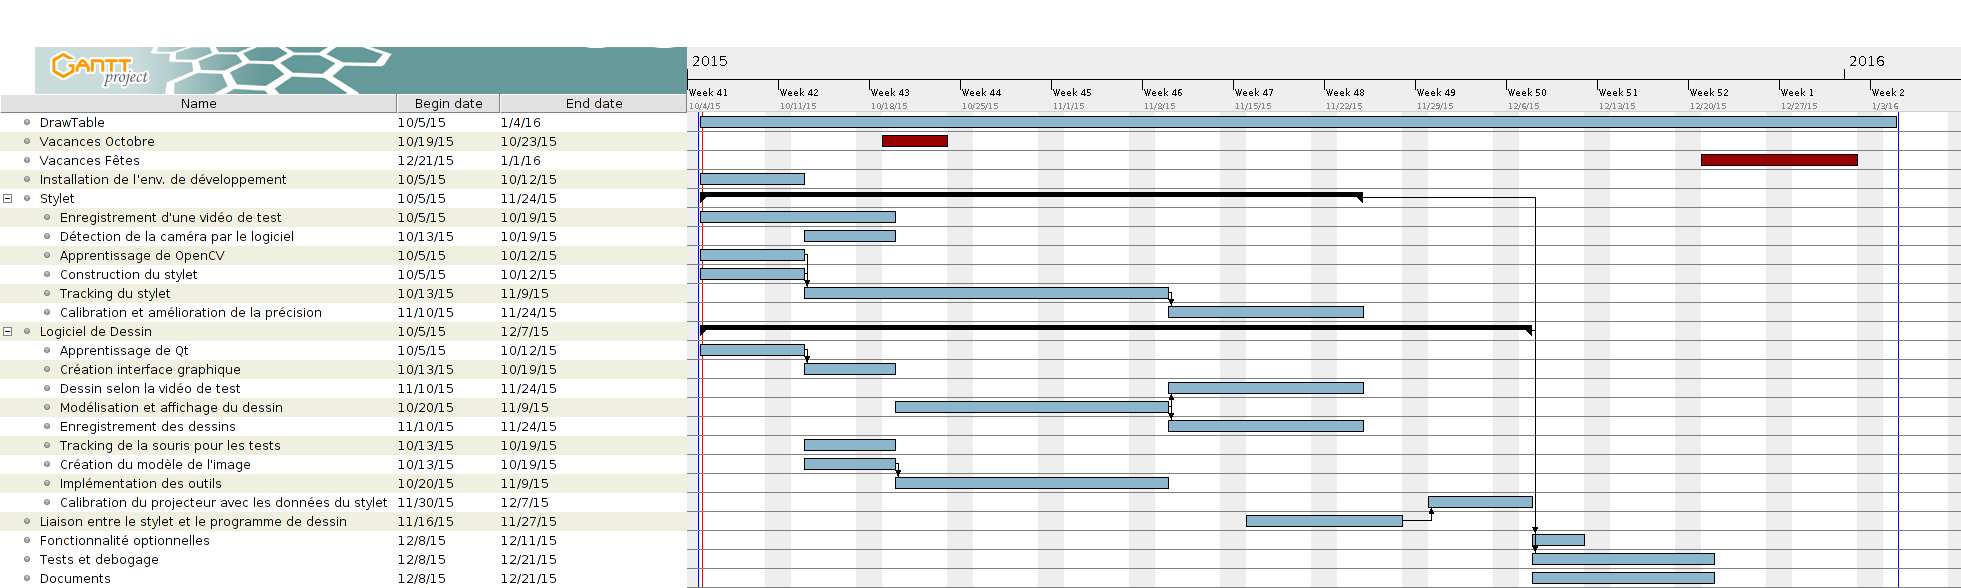
\includegraphics[angle=90, scale=0.35]{images/planification.png}
\caption{Planification initiale du projet}
\end{figure}

\newpage

\section{Planification finale}

\textit{TODO: définir la planification finale du projet avec Gantt Project.}

\end{document}